\documentclass[a4paper]{article}
\usepackage[english]{babel}
\usepackage[utf8]{vietnam}

%\usepackage{vntex}

%\usepackage[english,vietnam]{babel}
%\usepackage[utf8]{inputenc}

%\usepackage[utf8]{inputenc}
%\usepackage[francais]{babel}
\usepackage{a4wide,amssymb,epsfig,latexsym,multicol,array,hhline,fancyhdr}

\usepackage{amsmath}
\usepackage{lastpage}
\usepackage[lined,boxed,commentsnumbered]{algorithm2e}
\usepackage{enumerate}
\usepackage{color}
\usepackage{graphicx}		
\graphicspath{ {figures/} }
% Standard graphics package
\usepackage{listings}
\lstset{frame=tb,
  language=Python,
  aboveskip=3mm,
  belowskip=3mm,
  showstringspaces=false,
  columns=flexible,
  basicstyle={\small\ttfamily},
  numbers=none,
  numberstyle=\tiny\color{gray},
  keywordstyle=\color{blue},
  commentstyle=\color{dkgreen},
  stringstyle=\color{mauve},
  breaklines=true,
  breakatwhitespace=true,
  tabsize=3
}
\definecolor{dkgreen}{rgb}{0,0.6,0}
\definecolor{gray}{rgb}{0.5,0.5,0.5}
\definecolor{mauve}{rgb}{0.58,0,0.82}
\usepackage{array}
\usepackage{tabularx, caption}
\usepackage{multirow}
\usepackage{multicol}
\usepackage{rotating}
\usepackage{graphics}
\usepackage[a4paper,left=2cm,right=2cm,top=1.8cm,bottom=2.8cm]{geometry}
\usepackage{setspace}
\usepackage{epsfig}
\usepackage{tikz}
\usetikzlibrary{arrows,snakes,backgrounds}
\usepackage[bottom]{footmisc}
\usepackage[unicode]{hyperref}
\usepackage[labelformat=empty]{caption}

%can file puenc.def trong thu muc goc de option [unicode] tao ra bookmark bang tieng Viet
\hypersetup{urlcolor=blue,linkcolor=black,citecolor=black,colorlinks=true} 
%\usepackage{pstcol} 								
% PSTricks with the standard color package

\newtheorem{theorem}{{\bf Theorem}}
\newtheorem{property}{{\bf Property}}
\newtheorem{proposition}{{\bf Proposition}}
\newtheorem{corollary}[proposition]{{\bf Corollary}}
\newtheorem{lemma}[proposition]{{\bf Lemma}}


%\usepackage{fancyhdr}
\setlength{\headheight}{40pt}
\pagestyle{fancy}
\fancyhead{} % clear all header fields
\fancyhead[L]{
 \begin{tabular}{rl}
    \begin{picture}(25,15)(0,0)
    \put(0,-8){
\includegraphics[width=8mm, height=8mm]{hcmut.png}}
    %\put(0,-8){\epsfig{width=10mm,figure=hcmut.eps}}
   \end{picture}&
	%
\includegraphics[width=8mm, height=8mm]{hcmut.png} & %
	\begin{tabular}{l}
		\textbf{\bf \ttfamily Trường Đại học Bách Khoa - Đại học Quốc gia TP.HCM}\\
		\textbf{\bf \ttfamily Bộ môn Viễn Thông}
	\end{tabular} 	
 \end{tabular}
}
\fancyhead[R]{
	\begin{tabular}{l}
		\tiny \bf \\
		\tiny \bf 
	\end{tabular}  }
\fancyfoot{} % clear all footer fields
\fancyfoot[L]{\scriptsize \ttfamily Tự động phục hồi màu cho ảnh xám, 05/2021}
\fancyfoot[R]{\scriptsize \ttfamily {\thepage /ii}}
\renewcommand{\headrulewidth}{0.3pt}
\renewcommand{\footrulewidth}{0.3pt}

%%%
\setcounter{secnumdepth}{4}
\setcounter{tocdepth}{3}
\makeatletter
\newcounter {subsubsubsection}[subsubsection]
\renewcommand\thesubsubsubsection{\thesubsubsection .\@alph\c@subsubsubsection}
\newcommand\subsubsubsection{\@startsection{subsubsubsection}{4}{\z@}%
                                     {-3.25ex\@plus -1ex \@minus -.2ex}%
                                     {1.5ex \@plus .2ex}%
                                     {\normalfont\normalsize\bfseries}}
\newcommand*\l@subsubsubsection{\@dottedtocline{3}{10.0em}{4.1em}}
\newcommand*{\subsubsubsectionmark}[1]{}
\makeatother

\begin{document}

\begin{titlepage}

\begin{center}
TRƯỜNG ĐẠI HỌC BÁCH KHOA - ĐẠI HỌC QUỐC GIA TP.HCM\\
BỘ MÔN VIỄN THÔNG
\end{center}

\vspace{1cm}

\begin{figure}[h!]
\begin{center}

\includegraphics[width=3cm]{hcmut.png}
\end{center}
\end{figure}

\vspace{1cm}


\begin{center}
\begin{tabular}{c}
\multicolumn{1}{l}{\textbf{{\Large XỬ LÝ ẢNH}}}\\
~~\\
\hline
\\
\multicolumn{1}{l}{\textbf{{\Large Bài tập lớn}}}\\
\\
\textbf{\Huge Tự động phục hồi màu cho ảnh xám}\\
\\
\hline
\end{tabular}
\end{center}

\vspace{3cm}

\begin{table}[h]
\begin{tabular}{rrl}

\hspace{2.7 cm} & GVHD: TS. Võ Tuấn Kiệt & (kietvo@hcmut.edu.vn)\\\\
& Sinh viên: & Nguyễn Thành Trung - 1814515\\ && Nguyễn Thanh Trung - 1814514\\ && Nguyễn Tiến Dũng - 1811789\\ && Lê Huy - 1812361
\\\\\\\\\\\\\\\\

\end{tabular}
\end{table}

\begin{center}
{\footnotesize Hồ Chí Minh, 05/2021}
\end{center}
\end{titlepage}


%\thispagestyle{empty}
\pagenumbering{roman}

\newpage

\tableofcontents

\newpage

% \thispagestyle{empty}
\renewcommand{\listfigurename}{Danh sách hình minh hoạ}
\listoffigures

\newpage

\pagenumbering{arabic}
\fancyfoot[R]{\scriptsize \ttfamily {\thepage}/\pageref{LastPage}}

%%%%%%%%%%%%%%%%%%%%%%%%%%%%%%%%%
\section{Giới thiệu}

\subsection{Tổng quát}
Hiện nay, rất nhiều người có nhu cầu phục chế ảnh màu từ ảnh xám, những bức ảnh này thông thường là do tác động của thời gian bị làm mất hoặc sai màu. Một số khác là những bức ảnh được chụp ở thời xưa, lúc đó chưa có công nghệ chụp ảnh màu. Để thực hiện việc này, hầu hết mọi người đều sử dụng phương pháp thủ công là khôi phục bằng tay. Tuy hiện tại đã có sự giúp đỡ của các công cụ hỗ trợ chỉnh sửa hình ảnh, nhưng để có thể có một tấm ảnh đẹp yêu cầu người chỉnh sửa  mất nhiều thời gian, có thể lên đến hàng tháng đối với những bức ảnh có nhiều chi tiết.\\

\noindent
Thấy được những yêu cầu trên, nhóm em đã thử tìm kiếm các bài báo\footnote{Chi tiết trong phần \textbf{\nameref{references} tham khảo}} về cách thức có thể tự động phục chế màu cho ảnh bằng \textbf{máy học/học sâu} (\textit{Machine Learning/Deep Learning}). Từ đó xây dựng một mô hình tự động hoá việc tô màu ảnh.\\
Hầu hết ý tưởng cho mô hình của nhóm được tham khảo từ bài báo \href{https://arxiv.org/abs/1611.07004}{\textbf{Image-to-Image Translation with Condition Adversarial Networks}}, hay còn được biết với cái tên \textbf{pix2pix}, đưa ra giải pháp cho những vấn đề về image-to-image và một trong số đó có liên quan tới việc tô màu ảnh. 

\subsection{Mục tiêu}\label{objective}
Việc khôi phục màu cho ảnh đúng tuyệt đối như những gì được chụp là chuyện gần như bất khả thi vì không ai có thể biết được thực sự màu của những đối tượng cần được tô màu một cách chắc chắn. Hơn thế nữa, việc một đối tượng có thể có nhiều màu phù hợp là chuyện rất đỗi bình thường. Ví dụ đơn giản như một nải chuối có thể màu lục khi chưa chín nhưng lại cũng có thể là màu vàng khi chín và thậm chí có thể đã chín nhưng vẫn còn màu lục.

\begin{figure}[h!]
\centering
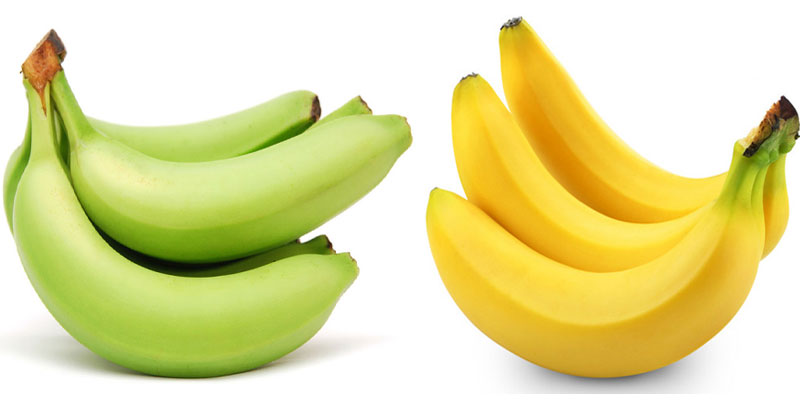
\includegraphics[width=15cm]{images/1_1.jpg}
\caption{Hình 1.1: Nải chuối có thể màu lục hoặc màu vàng. Nguồn: \href{https://bit.ly/3e7nqRs}{https://bit.ly/3e7nqRs}}
\end{figure}

\noindent
Nhưng không vì thế mà ta có thể tô bất cứ màu nào cho bất cứ đối tượng nào, giả sử như việc tô màu da người là màu xanh biển hoặc mặt trời thì màu xanh lá là không hợp lý.\\

\noindent
Từ đó cho thấy công việc phục hồi màu là một công việc thực sự rất khó khăn và cũng tràn đầy thú vị. Về vấn đề này, đã có không ít nghiên cứu cho ra nhiều phương pháp để hạn chế sự thủ công khi phục hồi màu cho ảnh suốt nhiều năm gần đây bằng cách tận dụng sức mạnh ngày càng lớn của \textbf{Trí tuệ nhân tạo} (\textit{Artificial Intelligence}).\\

\noindent
Trên những cơ sở đó, mục tiêu của nhóm khi lên kế hoạch tìm hiểu và thực hiện đề tài này là \textbf{xây dựng được một mô hình học sâu có thể dự đoán màu của những đối tượng trong ảnh xám một cách hợp lý} hơn là chính xác tuyệt đối. Chất lương dự đoán của mô hình cũng không mong đợi có thể bằng được so với làm thủ công, nhưng kết quả này sẽ giúp quá trình cải thiện chi tiết bằng thủ công được tiết kiệm thời gian hơn rất nhiều.

%%%%%%%%%%%%%%%%%%%%%%%%%%%%%%%%%
\section{Xử lí bài toán}

\subsection{Lựa chọn không gian màu}

\subsubsection{Không gian màu RGB}
Hầu hết khi làm việc với ảnh số (\textit{digital image}), ta sẽ thao tác với ảnh \textbf{RGB}, tức ảnh có 3 kênh màu đỏ-lục-lam (\textit{red-green-blue}). Mỗi điểm ảnh (\textit{pixel}) sẽ có 3 giá trị \textbf{R-G-B}, mỗi giá trị là một số nguyên nằm trong đoạn $[0, 255]$, tương ứng với 3 kênh màu để tạo nên được màu sắc của điểm ảnh đó.

\begin{figure}[h!]
\centering
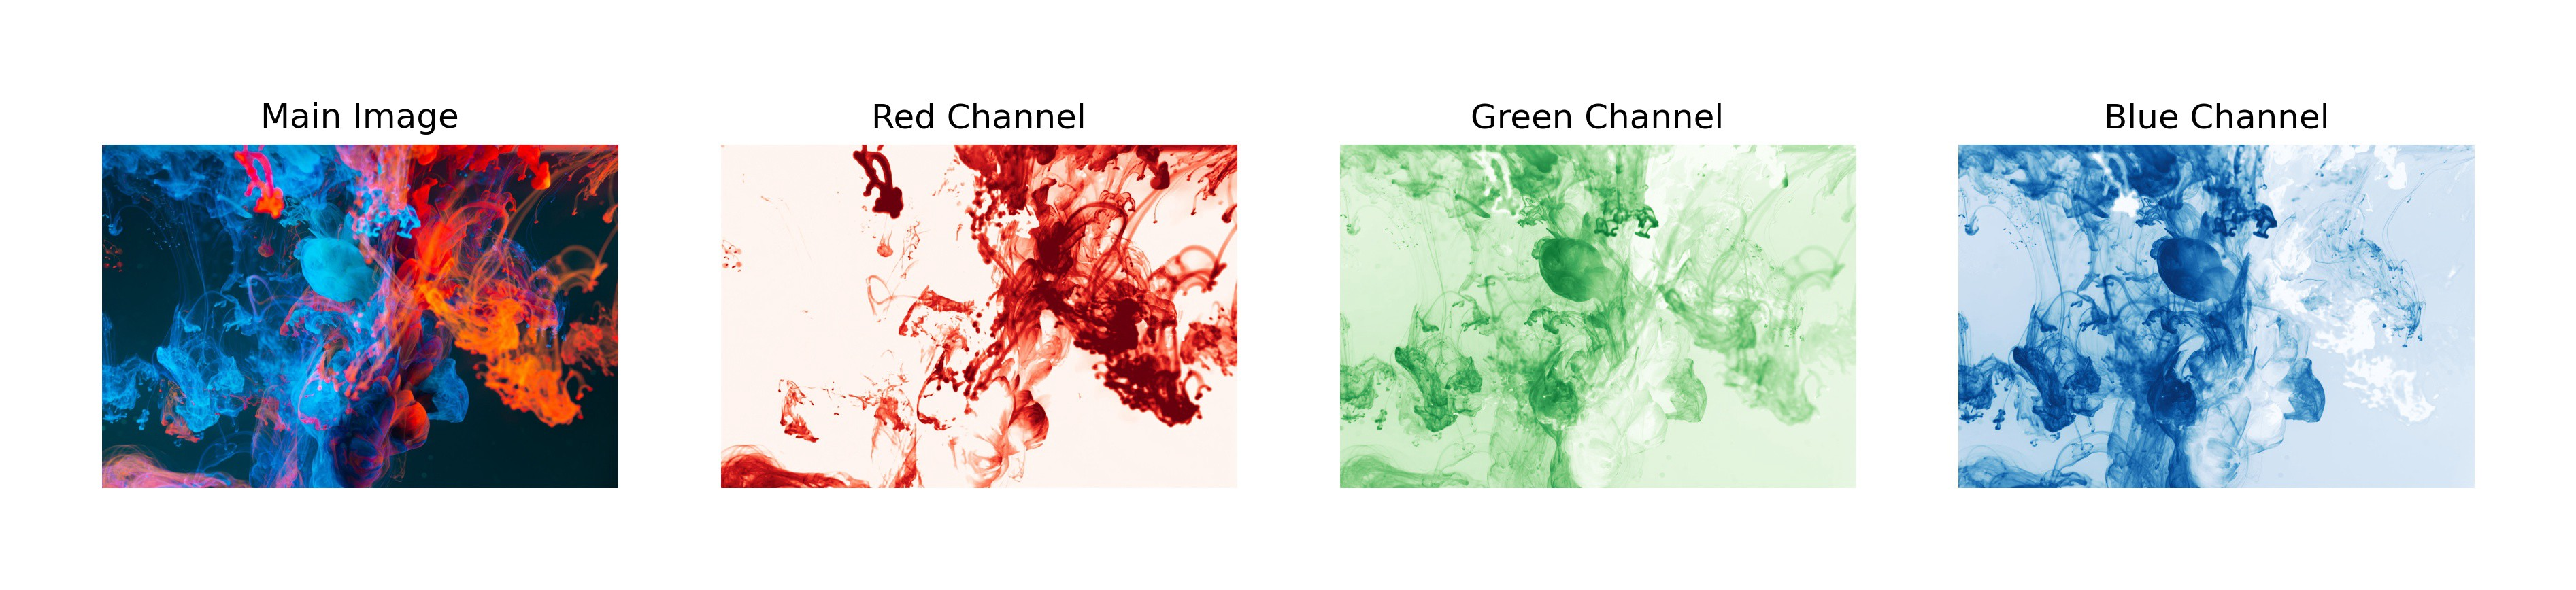
\includegraphics[width=16.1cm]{images/2_1.jpeg}
\caption{Hình 2.1: Các kênh màu đỏ, lục và lam được tách ra riêng biệt. Nguồn: \href{https://bit.ly/3eKaaBj}{https://bit.ly/3eKaaBj}}
\end{figure}

\subsubsection{Không gian màu Lab}
Ngoài RGB, một không gian màu khác cũng được sử dụng nhiều là không gian màu \textbf{Lab}, không gian này cũng quan tâm đến 3 thông số của mỗi điểm ảnh. Thông số đầu tiên là \textbf{L} (\textit{Lightness}) đại diện cho độ sáng của của mỗi điểm ảnh. hai thông số còn lại là \textbf{a} và \textbf{b} sẽ mang thông tin lần lượt là lục-đỏ (\textit{green-red}) và vàng-lam (\textit{yellow-blue}). Giá trị \textbf{a} càng nhỏ thì màu lục nhiều, màu đỏ ít. Ngược lại giá trị của\textbf{a} càng lớn thì màu lục ít, màu đỏ nhiều và tương tự với giá trị \textbf{b}.

\begin{figure}[h!]
\centering
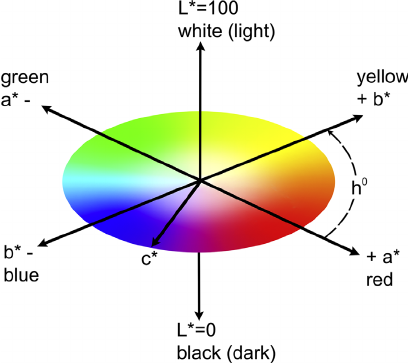
\includegraphics[width=5.8cm]{images/2_2.png}
\caption{Hình 2.2: Không gian màu Lab. Nguồn: \href{https://bit.ly/3nFIQIp}{https://bit.ly/3nFIQIp}}
\end{figure}

\noindent
Với thông số \textbf{L}, giá trị sẽ nằm trong đoạn $[0, 100]$. Riêng hai giá trị còn lại, không có cụ thể một khoảng nhất định, mà tuỳ thuộc vào phần mềm, chương trình mà ta sử dụng. Thường sẽ là khoảng $[-128, 127]$, tuy nhiên mô hình của nhóm không sử dụng khoảng giá trị trên. Chi tiết về vấn đề này sẽ được em làm rõ hơn ở phần \textbf{3.3 \nameref{normalization}}.

\begin{figure}[h!]
\centering
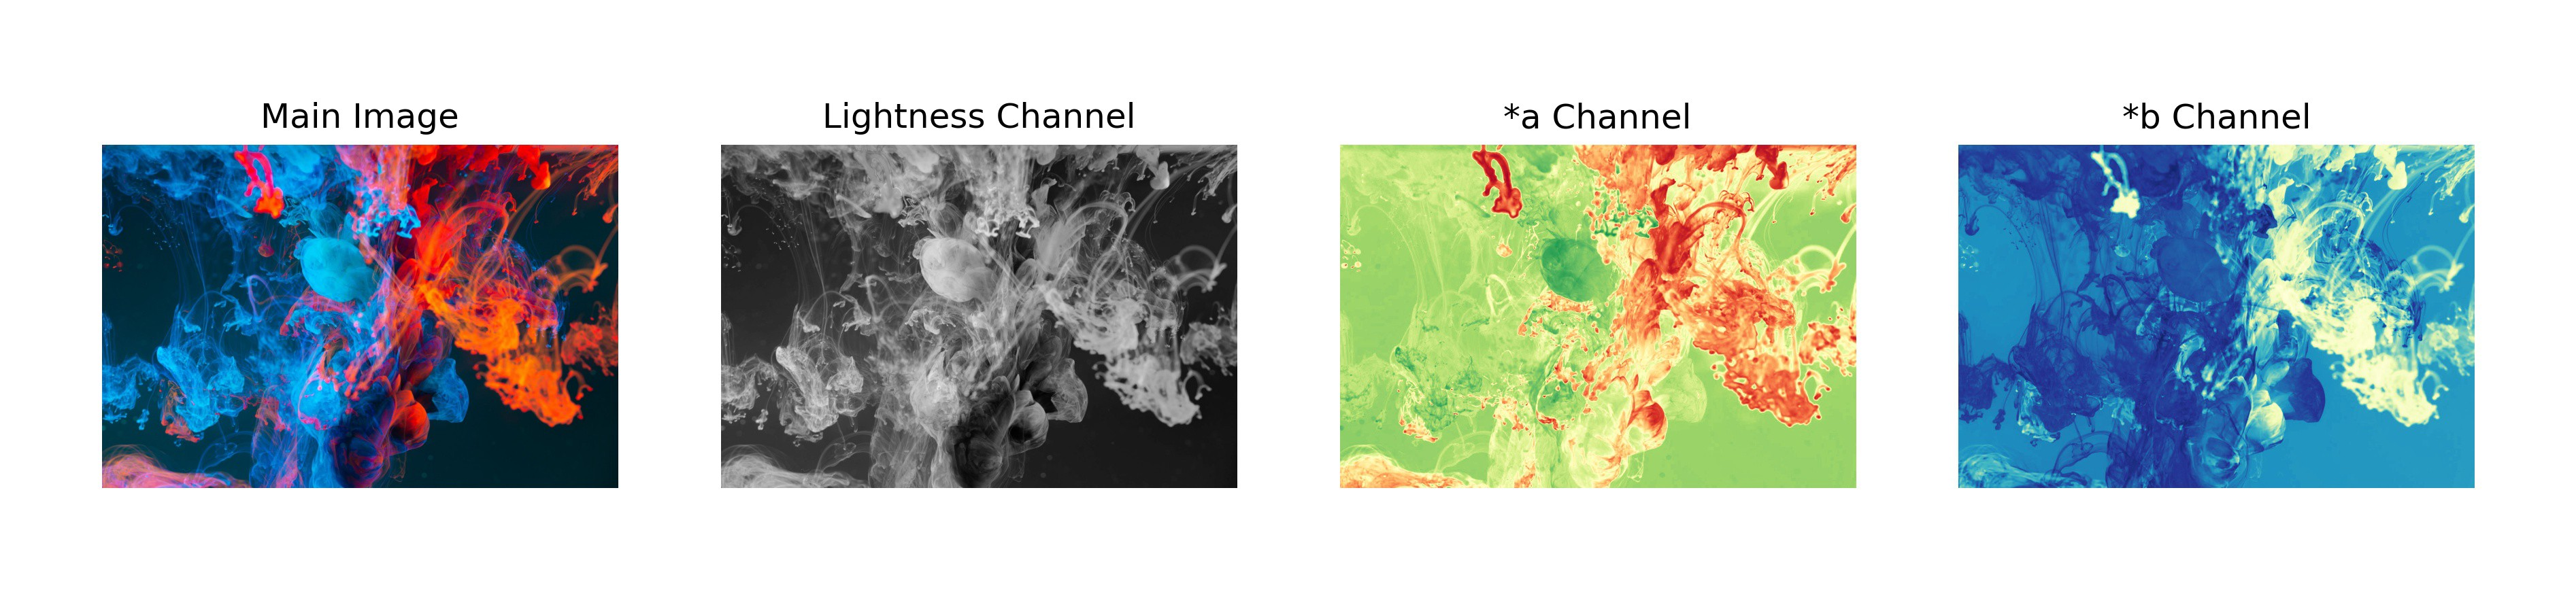
\includegraphics[width=16.1cm]{images/2_3.jpeg}
\caption{Hình 2.3: Các giá trị \textbf{L}, \textbf{a} và \textbf{b} được tách ra riêng biệt. Nguồn: \href{https://bit.ly/3eKaaBj}{https://bit.ly/3eKaaBj}}
\end{figure}

\subsubsection{Vì sao lựa chọn sử dụng không gian màu Lab thay vì RGB?}
Sau một thời gian tìm hiểu qua các bài báo xử lý vấn đề phục chế màu cho ảnh xám, nhóm nhận thấy rằng hầu như không ai sử dụng không gian màu RGB để giải quyết bài toán này mà thay vào đó là sử dụng không gian màu Lab. Lí do là khi sử dụng không gian màu Lab, sẽ có hai lợi thế:
\begin{enumerate}[i)]
    \item Không gian màu Lab được thiết kế để đồng nhất về cảm giác, điều này làm cho không gian màu này trở nên lý tưởng cho việc xử lý hình ảnh trên máy tính.
    
    \item Ta có thể tận dụng trực tiếp giá trị mức xám của ảnh đầu vào để tính toán thông số \textbf{L} bằng cách điều chỉnh tỉ lệ (\textit{scale}). Khi đó mô hình chỉ phải dự đoán giá trị 2 kênh \textbf{a} và \textbf{b} thay vì phải dự đoán cả 3 là \textbf{R}, \textbf{G} và \textbf{B}.
\end{enumerate}

\subsection{Một số phương pháp đơn giản}

\subsubsection{Đánh dấu màu vài điểm ảnh và dùng thuật toán lan}
Từ một tấm ảnh xám đầu vào, ta sẽ vẽ một vài màu cơ bản từ đó làm nền tảng, định hướng cho mô hình. Ý tưởng này xuất phát từ quan sát rằng, những điểm ảnh có độ sáng gần bằng nhau (mức xám xấp xỉ) và có khoảng cách trên ảnh gần nhau sẽ có khả năng tương tự cao dẫn đến màu giống nhau.

\begin{figure}[h!]
\centering
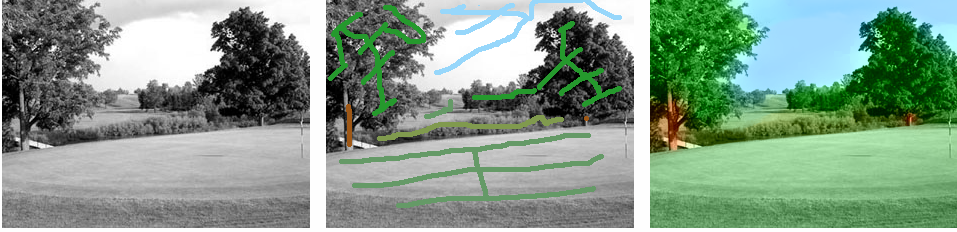
\includegraphics[width=15cm]{images/2_4.png}
\caption{Hình 2.4: Mô tả ý tưởng thuật toán đánh dấu vài điểm ảnh. Nguồn: \href{https://bit.ly/3eKdmwN}{https://bit.ly/3eKdmwN}}
\end{figure}

\subsubsection{Dựa vào màu sắc của ảnh có bố cục tương tự}
Ý tưởng thuật toán khá giống các bài toán phân loại (\textit{classification}), ta sẽ chọn ra một tấm ảnh có bố cục tương tự rồi dựa vào màu của ảnh đó kết hợp chỉnh sửa để đưa ra dự đoán.

\begin{figure}[h!]
\centering
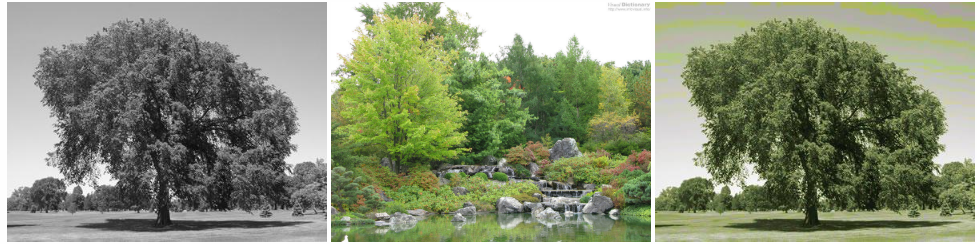
\includegraphics[width=15cm]{images/2_5.png}
\caption{Hình 2.5: Mô tả ý tưởng thuật toán ảnh có bố cục tương tự. Nguồn: \href{https://bit.ly/3eKdmwN}{https://bit.ly/3eKdmwN}}
\end{figure}

\noindent
Vì chưa thực sự tìm hiểu sâu về hai phương pháp trên, nên nhóm em xin phép không đi sâu vào phần cách thức thuật toán hoạt động.

\subsubsection{Hạn chế}
Cả hai phương pháp còn khá thủ công, chưa tự động được khi ta phải vẽ màu định hướng hoặc chọn ảnh có bố cục tương tự.\\
Với phương pháp \textbf{Đánh dấu màu vài điểm ảnh và dùng thuật toán lan} sẽ gặp khó khăn khi bức ảnh có nhiều chi tiết khác màu nhau thì sẽ gây nhiều khó khăn trong việc vẽ màu định hướng.\\
Việc tìm bố cục tương tự với bức ảnh đầu vào cũng là một bài toán không hề đơn giản, điều này khiến phương pháp \textbf{Dựa vào màu của ảnh có bố cục tương tự} trở nên bất khả thi khi chưa tìm được ảnh có bố cục tương tự ưng ý.

\subsection{Phương pháp sử dụng Mạng đối nghịch tạo sinh (GAN - Generative Adversarial Network) kết hợp mô hình mạng Unet}

Đây là phương pháp nhóm em đã chọn để xử lý cho bài toán này, để có thể hiểu được kiến trúc mô hình, ta sẽ xem xét những thành phần cơ bản của nó.

\subsubsection{Mạng đối nghịch tạo sinh - GAN}
Mạng GAN thuộc nhóm mô hình sinh dữ liệu mới. Dữ liệu sinh ra nhìn như thật nhưng không phải thật. Ví dụ như ảnh mặt người dưới đây là do GAN sinh ra, không phải mặt người thật.

\begin{figure}[h!]
\centering
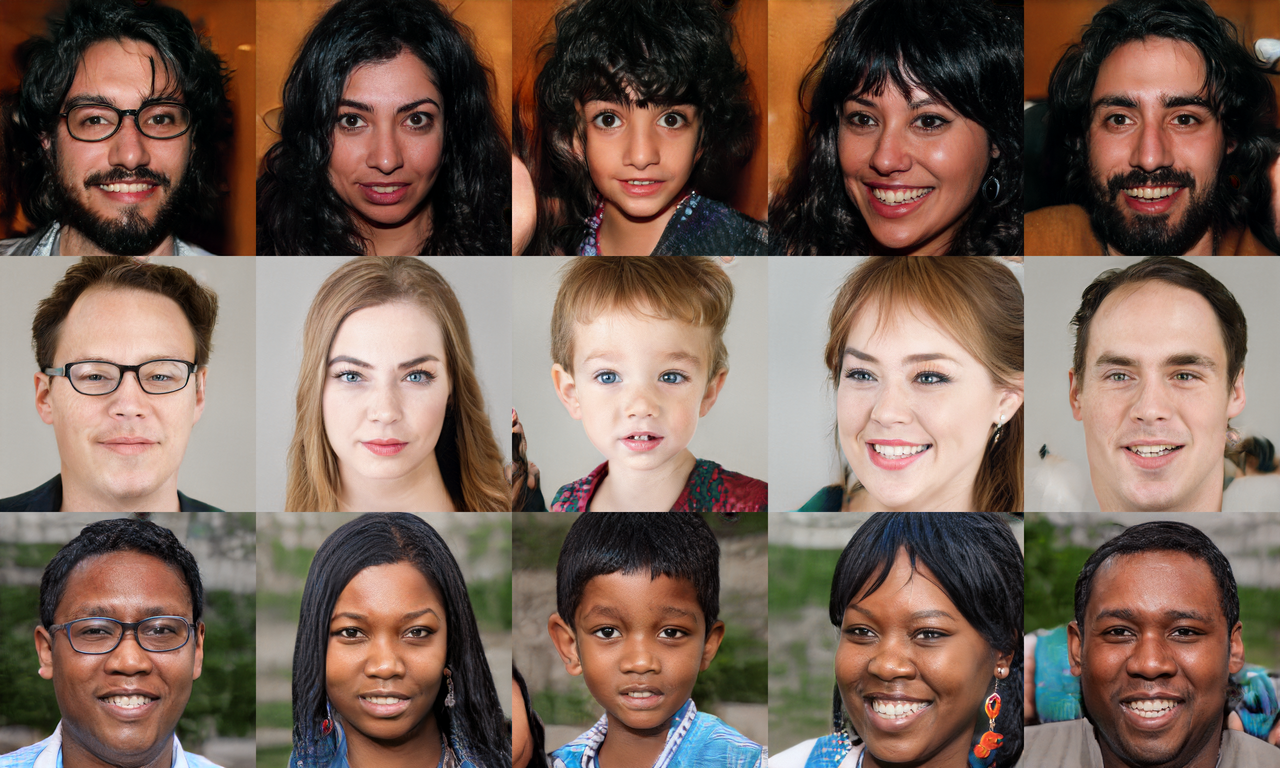
\includegraphics[width=13cm]{images/2_6.PNG}
\caption{Hình 2.6: Ảnh mặt người sinh ra bởi StyleGAN. Nguồn: \href{https://github.com/NVlabs/stylegan}{https://github.com/NVlabs/stylegan}}
\end{figure}

\noindent
G - \textbf{G}enerative ý chỉ sinh, N - \textbf{N}etwork là mạng, còn A - \textbf{A}dversarial là đối nghịch. Lí do là trong mạng này được tạo nên từ sự kết hợp giữa 2 mạng là \textbf{bộ sinh} (\textit{G - Generator}) và \textbf{bộ phân biệt} (\textit{D - Discriminator}, luôn luôn đối nghịch nhau trong quá trình huấn luyện.\\
Trong khi bộ sinh cố gắng sinh ra các dữ liệu giống như thật thì bộ phân biệt lại cố gắng phân biệt đâu là dữ liệu được sinh ra từ bộ sinh và đâu là dữ liệu thật.\\

\noindent
Giả sử như bài toán đưa cho GAN là sinh ra tiền giả giống như tiền thật để có thể dùng được, bộ sinh là người làm tiền giả, còn bộ phân biệt giống như cảnh sát. Người làm tiền giả sẽ cố gắng làm ra những tờ tiền giả sao cho cảnh sát không biết đó là tiền giả, còn cảnh sát thì cố gắng học để phân biệt được tiền nào là giả, tiền nào là thật.\\
Mục tiêu cuối cùng của GAN là người làm tiền giả phải có khả năng làm tiền giả sao cho cảnh sát không phân biệt được đâu là thật đâu là giả (50/50) để mang tiền giả đi tiêu thụ.\\
Trong quá trình huấn luyện mạng GAN thì nhiệm vụ của cảnh sát là học cách phân biệt tiền giả và tiền thật, bên cạnh đó là nói cho người làm tiền giả là nên làm giả như thế nào cho tốt hơn. Dần dần thì người làm tiền giả sẽ làm ra được tiền giống tiền thật và cảnh sát cũng trở nên thành thạo trong việc phân biệt tiền thật hay giả.\\

\noindent
Ý tưởng của GAN bắt nguồn từ \href{https://cs.stanford.edu/people/eroberts/courses/soco/projects/1998-99/game-theory/nonzero.html}{Non-Zero-Sum Games}\footnote{Stanford, \lq Non-Zero-Sum Games\rq, \href{https://stanford.io/3nCiLKq}{https://stanford.io/3nCiLKq}}, là một trò chơi đối kháng giữa 2 người, nếu một trong hai người thắng, thì người còn lại sẽ thua. Ở mỗi lượt, cả hai người đều muốn tối đa hoá cơ hội thắng của mình và tối thiểu hoá cơ hội thắng của đối phương. Trong lý thuyết trò chơi thì mô hình sẽ hội tụ khi cả bộ sinh và bộ phân biệt đạt tới trạng thái cân bằng Nash (\textit{Nash equilibrium}\footnote{Jørgen Veisdal, \lq The Nash equilibrium, explained\rq, \href{https://bit.ly/3ea57Lr}{https://bit.ly/3ea57Lr}}), tức là các bước tiếp theo của bất cứ ai trong hai người đều không làm thay đổi cơ hội thẳng của ai cả.

\begin{figure}[h!]
\centering
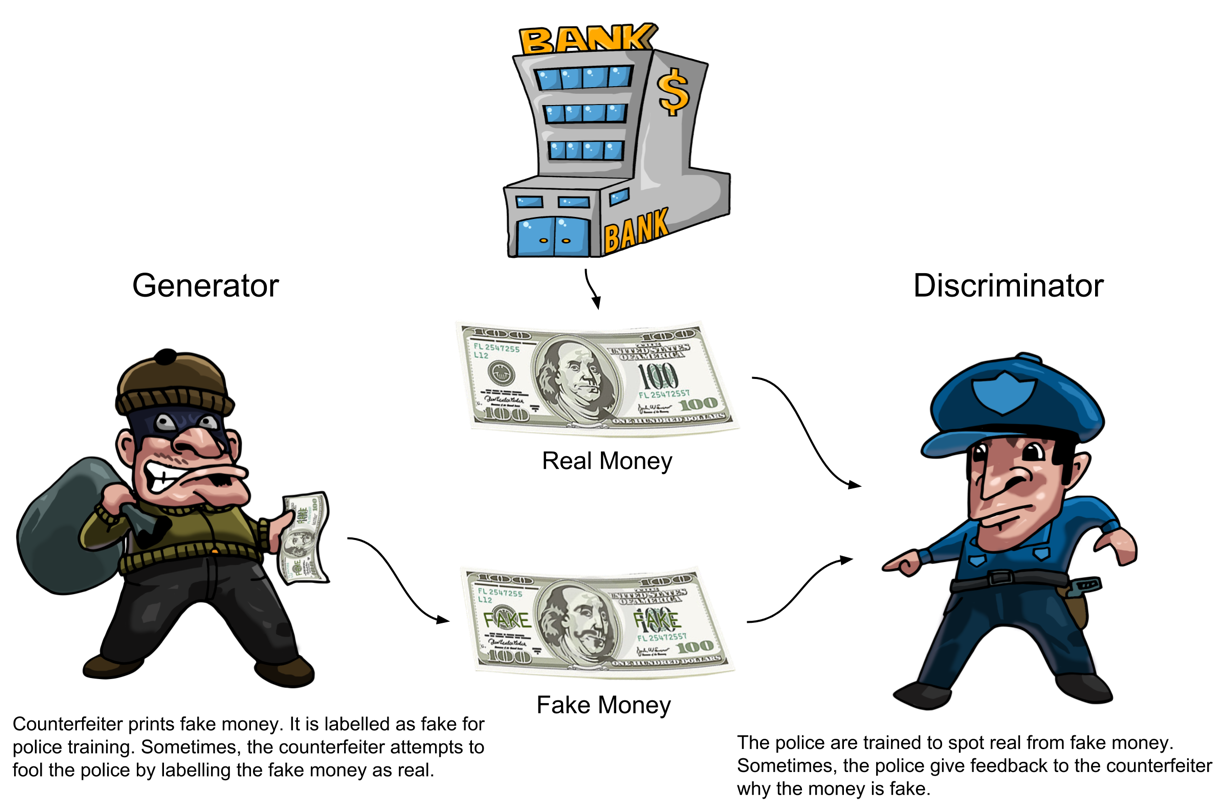
\includegraphics[width=9.5cm]{images/2_7.png}
\caption{Hình 2.7: Minh hoạ bộ sinh và bộ phân biệt trong mạng GAN. Nguồn: \href{https://bit.ly/3ue1M3r}{https://bit.ly/3ue1M3r}}
\end{figure}

\noindent
Nhìn theo khía cạnh kỹ thuật, một bộ sinh sẽ sinh ra dữ liệu tốt (dữ liệu mà chúng ta mong muốn) nếu ta không thể chỉ ra đâu là dữ liệu giả và đâu là dữ liệu thật. Trong thống kê, điều này được gọi là bài kiểm tra từ hai tập mẫu - một bài kiểm tra để trả lời câu hỏi liệu tập dữ liệu $X = \{x_1, x_2, \dots, x_n\}$ và $X'=\{x_1', x_2', \dots, x_n'\}$ có được rút ra từ cùng một phân phối hay không. Sự khác biệt chính giữa hầu hết những bài nghiên cứu thông kê và GAN, là GAN sử dụng ý tưởng này theo kiểu có tính xây dựng. Nói cách khác, thay vì chỉ huấn luyện mô hình để nói \textit{``này, hai tập dữ liệu đó có vẻ như không đến từ cùng một phân phối''}, thì GAN sử dụng phương pháp \textbf{kiểm tra trên hai tập mẫu}\footnote{Wikipedia, \lq Two-sample hypothesis testing\rq, \href{https://en.wikipedia.org/wiki/Two-sample\_hypothesis\_testing}{https://en.wikipedia.org/wiki/Two-sample\_hypothesis\_testing}} để cung cấp tín hiệu cho việc huấn luyện cho bộ sinh. Điều này cho phép ta cải thiện bộ sinh có thể sinh dữ liệu tới khi ra được thứ gì đó giống như dữ liệu thực. Ở mức tối thiểu nhất, nó cần lựa được bộ phân biệt, kể cả bộ phân biệt của ta là một mạng nơ-ron sâu (\textit{Deep Neural Network}) tân tiến nhất.

\begin{figure}[h!]
\centering
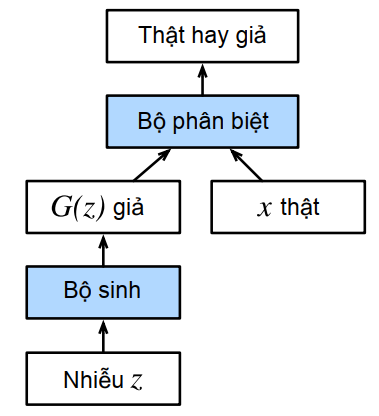
\includegraphics[width=6cm]{images/2_71.PNG}
\caption{Hình 2.8: Kiến trúc mạng đối nghịch tạo sinh}
\end{figure}

\noindent
Bộ phân biệt là một bộ phân loại nhị phân (\textit{binary classification}) nhằm phân biệt đầu vào $\mathbf{x}$ là thật (từ dữ liệu thật) hoặc giả (từ bộ sinh), được học theo kiểu có giám sát (\textit{supervised learning}). Thông thường, đầu ra của bộ phân biệt là một số vô hướng (\textit{scalar}) $o \in \mathbb{R}$ dự đoán cho đầu vào $\mathbf{x}$, và sẽ được đưa qua hàm sigmoid $S(x) = 1/(1+exp(-x)), R = (0, 1)$ để nhận được xác suất dự đoán với giá trị càng gần 1 thì bộ phân biệt càng có xu hướng quyết định đó là dữ liệu thật. Hàm mất mát của bộ phân biệt cũng vì thế mà có dạng entropy chéo, nghĩa là:
\begin{align*}
    \min_{D}\left\{-y\log D\left(\mathbf{x}\right) - \left(1-y\right)\log\left(1-D\left(\mathbf{x}\right)\right)\right\}
\end{align*}
Còn đối với bộ sinh, được học theo kiểu không giám sát (\textit{unsupervised learning}), trước tiên nó cần được cho vài tham số ngẫu nhiên được xem là nhiễu $\mathbf{z} \in \mathbb{R}^d$ (\textbf{số chiều $d$ thường là 100}\footnote{Reddit, ``Why is Z-dimension for GANs usually 100?'', \href{https://bit.ly/33nXNpk}{https://bit.ly/33nXNpk}}) từ một nguồn, ví dụ phân phối chuẩn $\mathbf{z} \sim \mathcal{N}\left(\mu, \sigma^2\right)=\mathcal{N}\left(0, 1\right)$. Mục tiêu của bộ sinh là đánh lừa bộ phân biệt để phân loại $\mathbf{x'} = G\left(\mathbf{z}\right)$ là dữ liệu thật, nghĩa là, ta muốn $D\left(G\left(\mathbf{z}\right)\right) \approx 1$. Nói cách khác, cho trước một bộ phân biệt $D$, ta sẽ cập nhật tham số của bộ sinh $G$ nhằm cực đại hoá mất mát entropy chéo khi $y=0$, tức là:
\begin{align*}
    \max_G\left\{-\log\left(1-D\left(G\left(\mathbf{z}\right)\right)\right)\right\}
\end{align*}
Tóm lại, $D$ và $G$ đang chơi trò ``minimax'' (cực tiểu hoá cực đại) với một hàm mục tiêu toàn diện như sau:
\begin{align*}
    \min_D\max_G\left\{-\mathbb{E}_{\mathbf{x}\sim \text{data}}\log D\left(\mathbf{x}\right)-\mathbb{E}_{\mathbf{z} \sim \text{noise}}\log\left(1-D\left(G\left(\mathbf{z}\right)\right)\right)\right\}\\
    \Leftrightarrow \min_G\max_D\left\{\mathbb{E}_{\mathbf{x}\sim \text{data}}\log D\left(\mathbf{x}\right)+\mathbb{E}_{\mathbf{z} \sim \text{noise}}\log\left(1-D\left(G\left(\mathbf{z}\right)\right)\right)\right\}
\end{align*}
Kí hiệu $\mathbb{E}$ ở đây chính là kì vọng toán, hiểu đơn giản là lấy trung bình của tất cả dữ liệu.

\begin{figure}[h!]
\centering
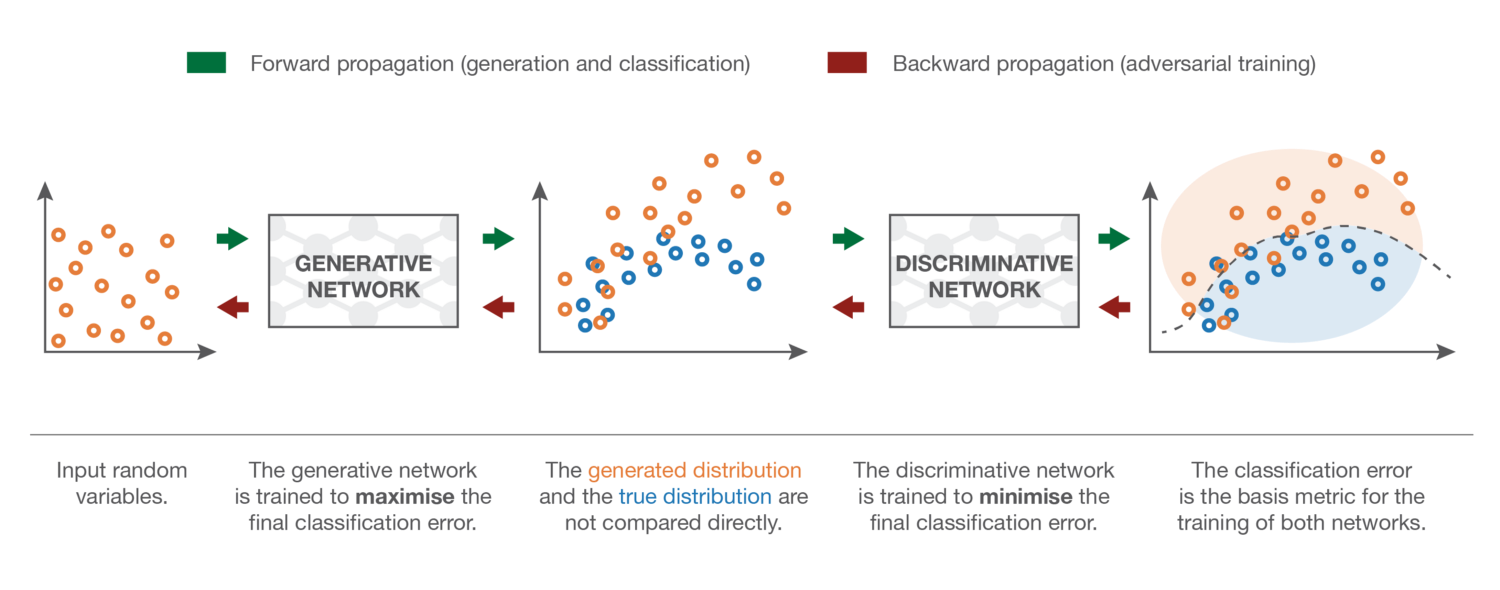
\includegraphics[width=16.5cm]{images/2_72.png}
\caption{Hình 2.9: Mô phỏng quá trình huấn luyện mạng GAN. Nguồn: \href{https://bit.ly/3vzdPIU}{https://bit.ly/3vzdPIU}}
\end{figure}

\subsubsection{Mô hình mạng Unet}
Unet là một kiến trúc được phát triển nhằm phân vùng các cấu trúc nơ-ron thần kinh trong não người. Kiến trúc này lần đầu được áp dụng đã giành chiến thắng trong cuộc thi EM segmentation challenge at ISBI 2012.\footnote{ISBS Challenge: Segmentation of neuonal structures in EM stacks, \href{http://brainiac2.mit.edu/isbi\_challenge/home}{http://brainiac2.mit.edu/isbi\_challenge/home}}

\noindent
Mạng Unet bao gồm 2 nhánh đối xứng nhau hình chữ U nên được gọi là Unet. Kiến trúc mạng bao gồm 2 phần là \textbf{thu hẹp} (\textit{contraction/encoder}) ở nhánh trái và \textbf{phần mở rộng} (\textit{expansion/decoder}) ở nhánh phải. Mỗi phần sẽ thực hiện một nhiệm vụ riêng như sau:

\begin{itemize}
    \item Phần thu hẹp: làm nhiệm vụ trích lọc đăc trưng để tìm ra bối cảnh của hình ảnh (\textit{WHAT}). Vai trò của phần thu hẹp tương tự như một encoder. Một mạng tích chập sâu sẽ đóng vai trò trích lọc đặc trưng. Lý do nhánh được gọi là thu hẹp vì kích thước dài và rộng của các tầng giảm dần, có thể hiểu là giảm độ phân giải (\textit{resolution}) bằng cách sử dụng \textbf{gộp cực đại} (\textit{max pooling}). Quá trình làm giảm kích thước còn được gọi là \textit{downsampling}.
    
    \item Phần mở rộng: Gồm các tầng đối xứng tương ứng với các tầng của nhánh thu hẹp. Quá trình làm tăng kích thước tầng gọi là \textit{upsampling}, hiểu theo một cách đơn giản là hàm ngược của tích chập (\textit{Deconvolution}) để tăng lại độ phân giải của ảnh để biết được vị trí (\textit{WHERE}) từ đó đánh dấu nhãn của từng điểm ảnh. Có nhiều phương pháp để giải chập, chẳng hạn như sao chép các giá trị điểm ảnh liền kề theo các kích thước cửa sổ hoặc một phương thức khác là sử dụng \textbf{tích chập giãn nở} (\textit{dilation convolution}). Nhưng được sử dụng nhiều nhất là \textbf{tích chập chuyển vị} (\textit{transposed convolution})
\end{itemize}

\noindent
Đặc trưng riêng trong cấu trúc của Unet đó là áp dụng những \textbf{kết nối tắt} (\textit{skip connection}) đối xứng giữa các tầng của nhánh bên trái tương ứng với các tầng bên nhánh bên phải.
\begin{figure}[h!]
\centering
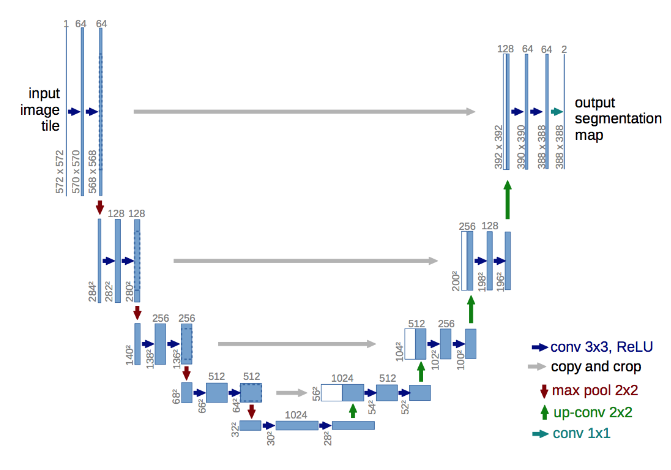
\includegraphics[width=10cm]{images/2_8.png}
\caption{Hình 2.10: Kiến trúc mô hình mạng Unet. Nguồn: \href{https://arxiv.org/abs/1505.04597}{https://arxiv.org/abs/1505.04597}}
\end{figure}

\noindent
Mô hình mạng Unet này sẽ được áp dụng vào bộ sinh trong mô hình mạng GAN. Hay nói cách khác, ta sẽ dùng mạng Unet để làm bộ sinh.

\subsection{Kiến trúc mô hình chính}
Với bài toán tô màu thì mục tiêu là từ đầu vào \textbf{L} (độ sáng - mức xám) của từng điểm ảnh ta sẽ dự đoán được cặp \textbf{(a, b)} để kết hợp tạo nên một tấm trong không gian màu Lab. Công việc này sẽ được bộ sinh đảm nhận.\\
Như vậy, để bộ phân biệt phát hiện được đâu là thật giả, ta cần phải đưa vào cho bộ phân biệt cả đầu vào lẫn đầu ra tức là cặp dữ liệu - nhãn. Đây chính là điều kiện xác suất cho dự đoán của bộ phân biệt và cũng chính là điểm khác biệt so với GAN thông thường, khi đó bộ phân biệt được nhìn thấy dữ liệu đầu vào thay vì chỉ mỗi bộ sinh.

\begin{figure}[h!]
\centering
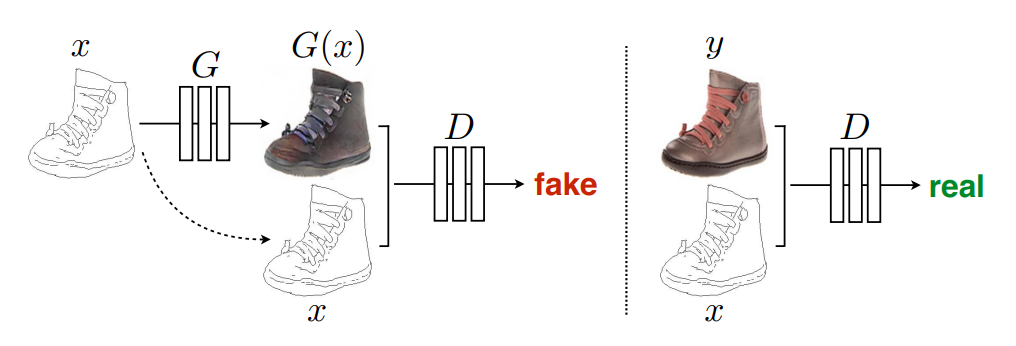
\includegraphics[width=13cm]{images/2_9.PNG}
\caption{Hình 2.11: Mô hình GAN dự đoán ảnh dựa vào đường viền. Nguồn: \href{https://arxiv.org/abs/1611.07004}{https://arxiv.org/abs/1611.07004}}
\end{figure}

\noindent
Do đó, hàm mất mát của mô hình GAN của chúng ta cũng sẽ khác biệt một chút so với một mạng GAN thông thường, cụ thể là:
\begin{align*}
    \mathcal{L}_{cGAN}(G, D) = \mathbb{E}_{\mathbf{x}, \mathbf{y}}\log D\left(\mathbf{x}, \mathbf{y}\right) + \mathbb{E}_{\mathbf{x}, \mathbf{z}}\log \left(1 - D\left(\mathbf{x}, G\left(\mathbf{x}, \mathbf{z}\right)\right)\right)
\end{align*}

\noindent
Trong đó, $\mathbf{x} \in \mathbb{R}^{1\times S \times S}$ là đầu vào chính là mức xám \textbf{L}, còn $y \in \mathbb{R}^{2\times S \times S}$ đầu ra là \textbf{(a, b)}. Nhiễu $\mathbf{z}$ được tạo ra từ việc \textbf{bỏ học} (\textit{dropout}).\footnote{Cụ thể được đề cập trong bài báo ``\textbf{Image-to-Image Translation with Conditional Adversarial Networks}'' là ``Instead, for our final models, we provide noiseonly in the form of dropout, applied on several layers of ourgenerator at both training and test time.''}\\
Nếu ta không dùng kỹ thuật bỏ học, mô hình vẫn sẽ có thể được huấn luyện và đưa ra kết quả dự đoán tốt tuy nhiên không được tổng quát, tức kết quả dự đoán của mô hình sẽ khá bị bó buộc khi phân phối sẽ chỉ có thể là hàm delta.\footnote{Cụ thể được đề cập trong bài báo ``\textbf{Image-to-Image Translation with Conditional Adversarial Networks}'' là ``Without $z$, the net could still learn a mapping from $x$ to $y$, but would produce deterministic outputs, and therefore fail to match any distribution other than a delta function.''}

\noindent
Một điểm khác biệt của bộ phân biệt trong mô hình này so với những bộ phân biệt trong các mô hình GAN thông thường là bộ phân biệt của chúng là bộ phân biệt cục bộ (\textit{Patch Discriminator}). Lí do là thay vì chỉ trả về là một đầu ra là một số vô hướng thì bộ phân biệt cục bộ sẽ trả về một ma trận $\mathbf{D} \in \mathbb{R}^{k\times k}$ bằng cách phân loại từng vùng $N \times N$ của đầu vào (ảnh có màu) là thật hay giả hay vì toàn bộ một lúc. Những vùng $N \times N$ này được gọi là vùng nhận thức (\textit{receptive field}) và phân loại mỗi vùng nhận thức sẽ cho một giá trị $\mathbf{D}_{ij}$. Kích thước của ma trận $\mathbf{D}$ (tức $k$) cũng như là vùng nhận thức (tức $N$) phụ thuộc vào các thông số của các tầng tích chập mà ta xây dựng cho bộ sinh, chi tiết sẽ được đề cập và làm rõ trong phần \textbf{3.4 \nameref{buildmodel}}.\\

\noindent
GAN hay chính xác hơn là bộ sinh sẽ làm nhiệm vụ giúp cho màu chúng ta dự đoán được đẹp, giống như thật. Không chỉ dừng lại ở đó, để có thể kiểm soát được chuyện mô hình tô màu được đẹp và giống thật, ta sẽ cho bộ sinh kết hợp với hàm mất mát dùng chuẩn 1 (\textit{norm 1} - L1 - \textit{mean absolute error}):
\begin{align*}
    \mathcal{L}_{L1}(G) = \mathbb{E}_{\mathbf{x}, \mathbf{y}, \mathbf{z}}\left|\left|\mathbf{y} - G(\mathbf{x}, \mathbf{z})\right|\right|_1
\end{align*}
Tại sao lại là chuẩn 1 thay vì chuẩn 2 (chuẩn Euclid)? Lí do là chuẩn 2 thường có ``trừng phạt'' mất mát nhiều hơn so với chuẩn 1, do đó điều này làm bó buộc kết quả dự đoán của bộ sinh làm cho mô hình có xu thế bảo thủ, sẽ dự đoán bằng cách lấy giá trị trung bình. Thay vì vậy, chuẩn 1 lại làm mềm việc ``trừng phạt'' này lại, khiến cho mô hình có thể sáng tạo để đưa ra dự đoán ``phiêu lưu'' hơn. \\
Cuối cùng, mô hình ta cần phải tối ưu là:
\begin{align*}
    G^* = \arg\underset{G}{\min}\underset{D}{\max}\mathcal{L}_{cGAN}(G, D) + \lambda \mathcal{L}_{L1}(G)
\end{align*}
Trong đó, $\lambda$ là hệ số cân bằng để giúp cho sự chênh lệch giữa hai hàm mất mát không bị áp đảo nghiêng về một bên, khiến một hàm bị ``lu mờ'' trong quá trình huấn luyện.\\
Thông thường giá trị hàm mất mát của GAN sẽ có giá trị lớn hơn nhiều so với hàm chuẩn 1. Nên xu hướng chọn $\lambda$ sẽ là một số khá lớn, và thường giá trị được chọn sẽ là $\lambda = 100$.

%%%%%%%%%%%%%%%%%%%%%%%%%%%%%%%%%
\section{Triển khai mô hình}

\subsection{Ngôn ngữ lập trình \& Thư viện chính}
Nhóm em sử dụng ngôn ngữ \textbf{Python} với sự hỗ trợ chính của thư viện \textbf{PyTorch}. Để cài đặt những công cụ này, có thể theo đường dẫn bên dưới:
\begin{itemize}
    \item Python: \href{https://www.python.org/downloads/}{https://www.python.org/downloads/}
    \item PyTorch \href{https://pytorch.org/get-started/locally/}{https://pytorch.org/get-started/locally/}
\end{itemize}
Bên cạnh đó, nhóm cũng sử dụng thêm thư viện \textbf{fastai} (bản mới nhất) cho việc xây dựng mạng Unet. Để cài đặt, ta sử dụng lệnh sau trong môi trường Python:
\begin{lstlisting}
pip install fastai --upgrade
\end{lstlisting}

\noindent
Toàn bộ mã nguồn, cũng như những tệp liên quan trong quá trình hoàn thành mô hình có thể tìm thấy tại:
\begin{itemize}
    \item Github: \href{https://github.com/dee-ex/EE3151\_SEM202\_PROJECT}{https://github.com/dee-ex/EE3151\_SEM202\_PROJECT}
\end{itemize}
Để có thể biết được đầy đủ những thư viện cũng như phiên bản thư viện được sử dụng, tham khảo tệp tin \texttt{requirements.txt}\footnote{Được chứa trong thư mục \href{https://github.com/dee-ex/EE3151\_SEM202\_PROJECT}{https://github.com/dee-ex/EE3151\_SEM202\_PROJECT}} trong đường dẫn phía trên.

\subsection{Tập dữ liệu}
Tập dữ liệu được nhóm chọn sử dụng là tập \href{https://cocodataset.org/#download}{\textbf{COCO}} có trong thư viện \textbf{fastai}, ta có thể dễ dàng tải về. Nhóm quyết định chọn $10,000$ ảnh để huấn luyện, còn quá trình xác thực sẽ là $2,000$.\\
Mô hình được chia ra huấn luyện hai giai đoạn. Giai đoạn đầu tiên là tiền huấn luyện, sẽ chỉ huấn luyện riêng bộ sinh với hàm mất mát $\mathcal{L}_{L1}$. Lúc này, ta dùng $2,000$ tấm ảnh cho việc xác thực để đưa ra mô hình phù hợp cho giai đoạn huấn luyện sau. Giai đoạn tiếp theo là huấn luyện GAN, vì yêu cầu mô hình sẽ là  tô màu cho ảnh một cách hợp lý chứ không phải chính xác tuyệt đối, chỉ một vài tấm ảnh được lấy ra trong tập xác thực sẽ được đánh giá kết quả tô màu qua từng epoch để quyết định lựa chọn mô hình cuối cùng.\\
Riêng với phần thử nghiệm, dữ liệu sẽ được nhóm chọn để có thể chủ động trong việc lựa chọn bố cục cho ảnh, từ đó có đánh giá đa dạng nhất cho mô hình.

\begin{figure}[h!]
\centering
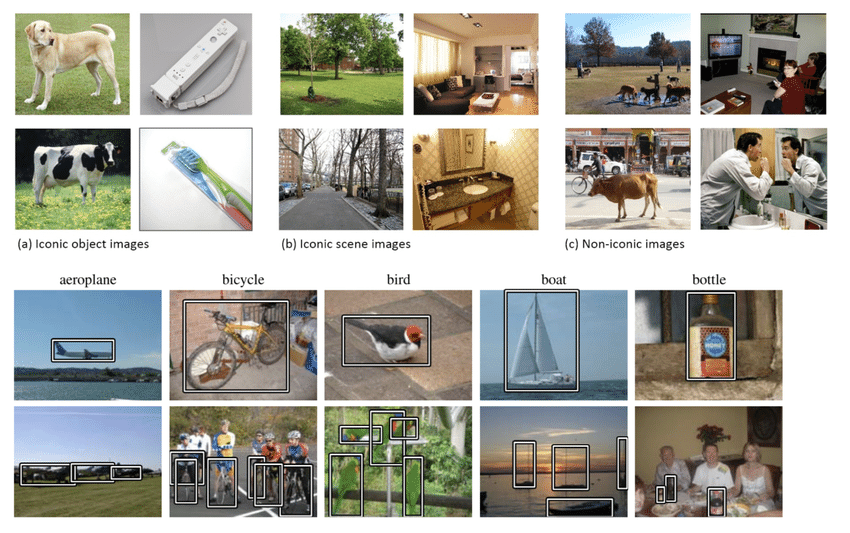
\includegraphics[width=12cm]{images/3_1.png}
\caption{Hình 3.1: Hình ảnh trích từ tập dữ liệu COCO}
\end{figure}

\subsection{Chuẩn hoá dữ liệu}\label{normalization}
\noindent
Khi sử dụng Pytorch để xử lý hình ảnh nhờ vào thư viện \texttt{PIL} và \texttt{skimage}, thì khoảng giá trị của không gian màu xám khi đưa về Tensor sẽ là $[0, 1]$, còn không gian màu Lab sẽ là:

\begin{itemize}
    \item \textbf{L} $\in [0, 100]$
    
    \item \textbf{a} $\in [-86.1830, 98.2331]$
    
    \item \textbf{b} $\in [-107.8573, 94.4781]$
\end{itemize}

\noindent
Ta có thể kiểm tra chuyện đó bằng cách:
\begin{lstlisting}
In [2]: import numpy as np
In [3]: colors = np.mgrid[0:256, 0:256, 0:256].astype(np.uint8)
In [4]: colors.shape
Out[4]: (3, 256, 256, 256)

In [6]: all_rgb = np.transpose(colors)
In [7]: from skimage import color
In [8]: all_lab = color.rgb2lab(all_rgb)
In [9]: np.max(all_lab, axis=(0, 1, 2))
Out[9]: array([100.        ,  98.23305386,  94.47812228])

In [10]: np.min(all_lab, axis=(0, 1, 2))
Out[10]: array([   0.        ,  -86.18302974, -107.85730021])
\end{lstlisting}

\noindent
Nhóm quyết định sẽ chuẩn hoá cả đầu vào và đầu ra nằm trong khảong $[-1, 1]$ để áp dụng hàm kích hoạt đầu ra là hàm $\tanh; \sigma(z) = \left(e^z-e^{-z}\right)/\left(e^z+e^{-z}\right), R = (-1, 1)$. Vậy nên, công thức chuẩn hoá sẽ là
\begin{align*}
    \textbf{L}_{\text{normalization}} = \dfrac{\textbf{L}}{50} - 1\\
    \textbf{(a, b)}_{\text{normalization}} = \dfrac{\textbf{(a, b)}}{110}
\end{align*}

\noindent
Bên cạnh đó, kích thước ảnh cũng sẽ được điều chỉnh (\textit{resize}) lại thành ảnh vuông kích thước $256\times 256$.

\subsection{Xây dựng mô hình}\label{buildmodel}

\subsubsection{Bộ sinh}
\begin{figure}[h!]
\centering
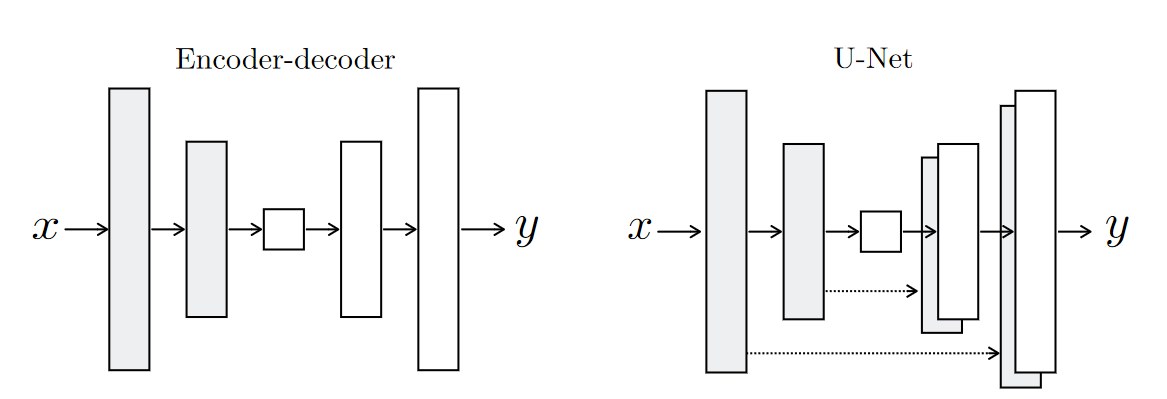
\includegraphics[width=10cm]{images/3_2.PNG}
\caption{Hình 3.2: Một trong 2 lựa chọn cho bộ sinh. Mô hình Encoder-Decoder trái, Unet phải}
\end{figure}

\noindent
Tổng quát, bộ sinh sẽ nhận đầu vào là một tập gồm $M \in \mathbb{N}^*$ ảnh xám kích thước $(S, S) = 256\times 256$, tức là một Tensor $\mathbf{X} \in \mathbb{R}^{M\times 1 \times S \times S}$. Đầu ra của bộ sinh là một Tensor $\mathbf{Y} \in \mathbb{R}^{M\times 2 \times S \times S}$.

\noindent
Giả sử \texttt{Ck} là khối Convolution-BatchNorm-ReLU với $k$ \textbf{bộ lọc} (\textit{kernel/filter}). \texttt{CDk} là khối Convolution-BatchNorm-Dropout-ReLU với tỉ lệ dropout là $50\%$ và $k$ bộ lọc. Tất cả đều sử dụng bộ lọc kích thước $4\times 4$ với \textbf{sải bước} (\textit{stride}) là $2$ và \textbf{đệm} (\textit{padding}) là $1$.\\
Sau mỗi khối \texttt{Ck} sẽ là một khối gộp cực đại để giảm kích thước (không tính chiều sâu) dữ liệu xuống gấp đôi. Còn sau mỗi khối \texttt{CDk} sẽ là một khối giải chập thì kích thước (không tích chiều sâu) dữ liệu tăng gấp đôi.\\
Cụ thể, mô hình sẽ có kiến trúc như chi tiết như sau:

\begin{itemize}
    \item \textbf{encoder:} \texttt{C64-C128-C256-C512-C512-C512-C512-C512}
    
    \item \textbf{decoder:} \texttt{CD512-CD1024-CD1024-C1024-C512-C256-C128}
\end{itemize}

\noindent
Ở \textbf{encoder}, ta sẽ sử dụng hàm LeakyReLU với độ dốc âm (\textit{negative slope}) là $0.2$ thay cho ReLU. Tầng cuối cùng của bộ sinh sẽ là một hàm $\tanh$. Một ngoại lệ là ở tầng đầu tiên ở \textbf{encoder} ta sẽ không sử dụng BatchNorm. Ta có lưu ý nhỏ ở đây, bản thân BatchNorm đã có bias nên là những tầng tích chập không cần phải có bias.\footnote{Stack Overflow - Patwie, ``Can not use both bias and batch normalization in convolution layers'', \href{https://bit.ly/3f25eb2}{https://bit.ly/3f25eb2}}

\subsubsection{Bộ phân biệt $70 \times 70$}
Nhìn chung, bộ phân biệt thường không có kiến trúc quá phức tạp (nhiều tầng) và mô hình này cũng không phải là ngoại lệ. Bộ sinh sẽ gồm các khối:

\begin{itemize}
    \item \texttt{C64-C128-C256-C512}
\end{itemize}

\noindent
Thêm một lưu ý ở đây là ở khối tích chập \texttt{C512} thì sải bước là 1. Sau đó, ta sẽ đưa kết quả đó qua thêm 1 tầng tích chập với chỉ một bộ lọc để đưa về một Tensor dạng $(N, 1, 30, 30)$ và sải bước vẫn tiếp tục là 1.\\
Với kiến trúc như trên, ta sẽ được vùng nhận thức $N \times N$ là $70 \times 70$. Đây là vùng nhận thức có kết quả thực nghiệm tốt nhất mà bài báo \textbf{pix2pix} đã chỉ ra.

\noindent
Để tính kích thước vùng nhận thức ở tầng thứ $l$ bất kì thì ta sẽ có công thức:\footnote{Github - phillipi, ``receptive\_field\_sizes.m'', \href{https://github.com/phillipi/pix2pix/blob/master/scripts/receptive\_field\_sizes.m}{https://github.com/phillipi/pix2pix/blob/master/scripts/receptive\_field\_sizes.m}}
\begin{align*}
    K_{l-1} = K + s_{l-1}(K_{l} - 1)
\end{align*}
Trong đó $K_l$ là kích thước vùng nhận thức ở tầng thứ $l$, $K$ là kích thước bộ lọc và $s_{l}$ chính là số sải bước ở tầng thứ $l$.

\begin{figure}[h!]
\centering
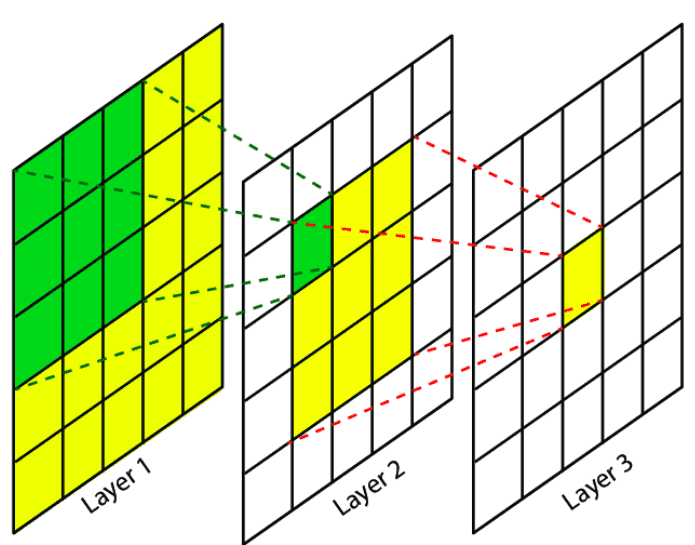
\includegraphics[width=6cm]{images/3_3.png}
\caption{Hình 3.3: Mô tả vùng nhận thức qua các tầng. Nguồn: \href{https://bit.ly/3xGaeLa}{https://bit.ly/3xGaeLa}}
\end{figure}

\noindent
Như vậy, với mỗi đầu ra $1 \times 1$ của kết quả $30\times 30$ thì kích thước vùng nhận thức quét được có thể được tính như sau:
\begin{align*}
    K_4 &= K + s_4(K_5 - 1) = 4 + 1(1-1) = 4\\
    K_3 &= K + s_3(K_4 - 1) = 4 + 1(4-1) = 7\\
    K_2 &= K + s_2(K_3 - 1) = 4 + 2(7-1) = 16\\
    K_1 &= K + s_1(K_2 - 1) = 4 + 2(16-1) = 34\\
    K_0 &= K + s_0(K_1 - 1) = 4 + 2(34 - 1) = 70
\end{align*}


\subsubsection{Học chuyển tiếp (Transfer learning)}
Sau khi huấn luyện mô hình và thử nghiệm thì thấy kết quả không được khả quan cho lắm.\footnote{Sẽ được trình bày trong phần \textbf{4 \nameref{testmodel}}}Do đó, nhóm đã quyết định tìm kiếm một mạng Unet được huấn luyện sẵn. Một trong những giải pháp được áp dụng phổ biến đó là sử dụng mạng \textbf{Resnet} (\textit{\textbf{Res}idual \textbf{Net}work}) cho phần thu hẹp (phía trái chữ U). Lí do là mạng ResNet cũng sử dụng những kết nối tắt trong kiến trúc của nó, phù hợp với kiến trúc mạng Unet. Ngoài ResNet, một mạng khác cũng có thể được áp dụng đó là \textbf{DenseNet}. Tuy nhiên, mạng \textbf{ResNet18} là lựa chọn cuối cùng do mô hình mạng có kích thước vừa phải, thuận tiện và thích hợp cho việc huấn luyện đối với phần cứng hiện tại của nhóm em.\\
Về phía phải chữ U, phần mở rộng, thư viện \texttt{fastai} cung cấp công cụ để có thể tự động xây dựng phần tương ứng với phần thu hẹp.

\begin{figure}[h!]
\centering
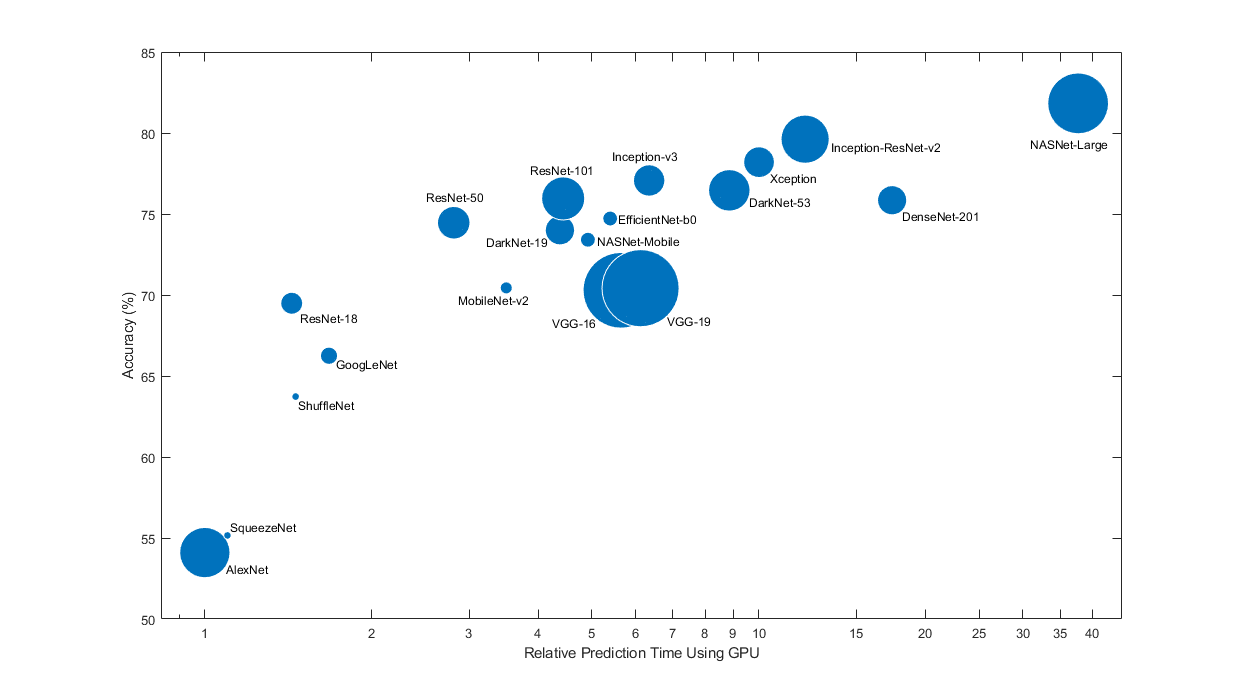
\includegraphics[width=16cm]{images/3_4.png}
\caption{Hình 3.4: So sánh các mô hình mạng tích chập hiện đại hiện nay}
\end{figure}

\subsubsection{Tiền huấn luyện độc lập bộ sinh ResNet}
Khi huấn luyện GAN, việc khó hơn cả là huấn luyện cho bộ sinh có thể sinh được dữ liệu ta mong muốn. Để tối ưu việc đó, ta sẽ đưa riêng ra huấn luyện bộ sinh trước khi đưa vào GAN nhờ vào hàm mất mát $\mathcal{L}_{\text{L1}}(G)$.\\

\noindent
Việc huấn luyện, nhóm sử dụng thuật toán tối ưu Adam với tốc độ học $\alpha =  10^{-4}$, tốc độ phân rã (\textit{exponential decay rates}) $\beta_1 = 0.9, \beta_2 = 0.999$ và $\epsilon = 10^{-8}$. Cho chạy batch size là 16 và 30 epoch. Mỗi epoch mất khoảng 6-7 phút (chưa tính phần xác thực).

\begin{figure}[h!]
\centering
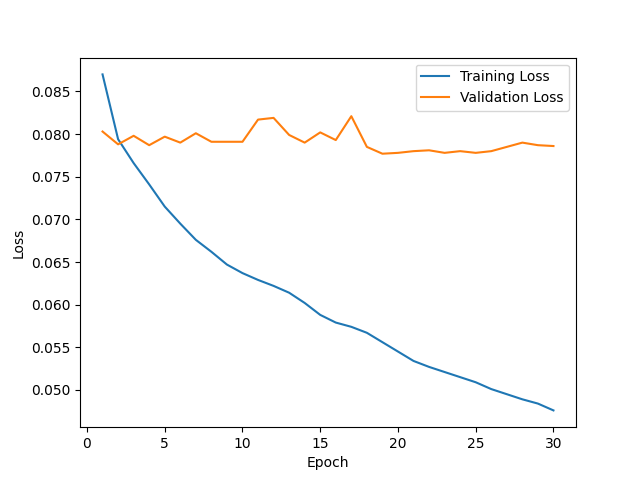
\includegraphics[width=10cm]{images/3_5.png}
\caption{Hình 3.5: Giá trị mất mát của bộ sinh trên hai tập huấn luyện \& xác thực qua từng epoch}
\end{figure}

\noindent
Dựa vào \textbf{Hình 3.5}, giá trị mất mát của mô hình không cao. Bên cạnh đó, ta thấy rằng giá trị mất mát trên tập huấn luyện có xu hướng giảm và tiếp tục giảm, còn giá trị mất mát trên tập xác thực thì có vẻ đã bão hoà. Để tránh \textbf{quá khớp} (\textit{overfitting}), nhóm em sẽ chọn mô hình thứ 20 (tức sau khi huấn luyện qua 20 epoch).

\subsubsection{Huấn luyện mạng GAN với bộ sinh ResNet}
Tải các thông số của bộ sinh đã được tiền huấn luyện độc lập trước đó, sau đó đưa vào để huấn luyện chung với bộ phân biệt với hệ số cân bằng $\lambda = 100$. Thuật toán tối ưu vẫn sẽ dùng là Adam để tối ưu bộ phân biệt ($D$) và bộ sinh ($G$) với các thông số được chọn là:
\begin{align*}
\alpha = 2\times 10^{-4}, \beta = (0.5, 0.999), \epsilon = 10^{-8}
\end{align*}
Cho chạy với batch size là 16 và 20 epoch. Mỗi epoch mất khoảng 10-16 phút (chưa tính phần xác thực).

\begin{figure}[h!]
\centering
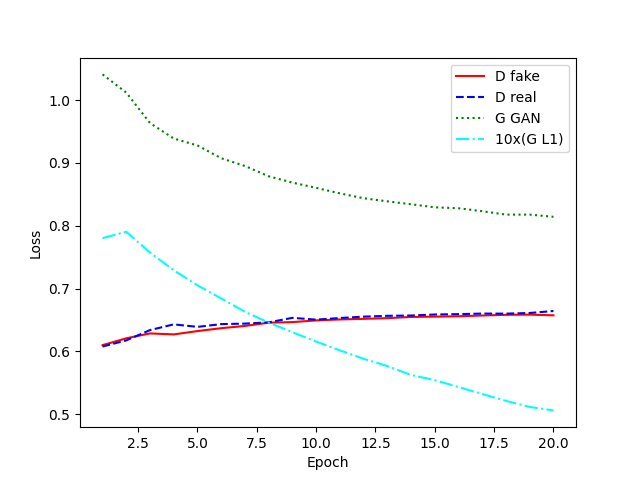
\includegraphics[width=10cm]{images/3_6.png}
\caption{Hình 3.6: Giá trị các thành phần mất mát của bộ phân biệt và bộ sinh qua từng epoch}
\end{figure}

\noindent
Nhận thấy xu hướng của giá trị mất mát khi huấn luyện mô hình GAN là giá trị mất mát của bộ phân biệt tăng thì giá trị mất mát của bộ sinh sẽ giảm và cả hai \textit{dường như} (chưa qua kiểm tra thực nghiệm) đều sẽ hội tụ về một giá trị. Lí giải điều này, khi bộ phân biệt đạt đến một ngưỡng thông minh nhất định, bộ sinh thì lại càng thông minh qua mỗi epoch hiển nhiên sẽ đánh lừa (\textit{fool}) được bộ phân biệt. Điều này phù hợp với nguyên lí \textbf{non-zero-sum-games}. Ngoài ra, giá trị mất mát của bộ sinh theo chuẩn 1 cũng được giảm, tuy không đáng kể.\\

\noindent
Sau khi xem xét một vài kết quả của mô hình sau mỗi epoch,\footnote{Sẽ được trình bày trong phần \textbf{4 \nameref{testmodel}}} em quyết định chọn mô hình thứ 15 (tức sau khi huấn luyện qua 15 epoch).

%%%%%%%%%%%%%%%%%%%%%%%%%%%%%%%%%
\section{Thử nghiệm mô hình}\label{testmodel}\label{experiment}

\subsection{Mô hình GAN với bộ sinh đơn giản kết hợp chuẩn 1}

\begin{figure}[h!]
\centering
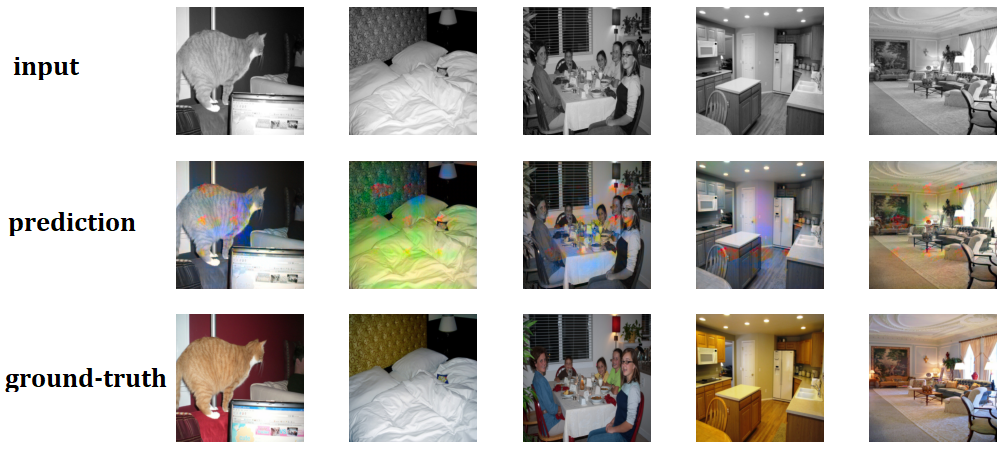
\includegraphics[width=15cm]{images/4_0.png}
\caption{Hình 4.1: Kết quả dự đoán của mô hình GAN với bộ sinh đơn giản kết hợp chuẩn 1 trên dữ liệu xác thực của tập dữ liệu \textbf{COCO} sau epoch thứ 34}
\end{figure}

\noindent
Cơ bản, việc huấn luyện mô hình là khả thi khi mô hình cũng đã có thể tô được màu sau vài chục epoch. Nhưng giới hạn về phần cứng cũng như là tập dữ liệu không đủ nhiều và tốt để có thể huấn luyện được mô hình một cách trọn vẹn.\\
Bản thân việc huấn luyện một mạng GAN cũng không dễ dàng khi GAN rất nhạy cảm với những \textbf{thông số cấu trúc} (\textit{hyperparameter}). Sau nhiều lần thử nghiệm thất bại, nhóm em cũng đã rút ra một vài kinh nghiệm khi huấn luyện GAN. Một trong số đó như là việc trong hầu hết các mô hình GAN, ta có thể khởi tạo các \textbf{trọng số} (\textit{weight}) và bias theo phân phối chuẩn $\mathcal{N}\left(\mu, \sigma^2\right) = \mathcal{N}\left(0, 1\right)$ để quá trình huấn luyện có kết quả được nhanh hơn.\\

\noindent
Do những hạn chế trên, nhóm đã chuyển phương hướng thay vì xây dựng một bộ sinh từ đầu thì sẽ tận dụng khả năng học chuyển tiếp để tận dụng những mô hình có sẵn.

\subsection{Mô hình GAN với bộ sinh ResNet kết hợp chuẩn 1}

\begin{figure}[h!]
\centering
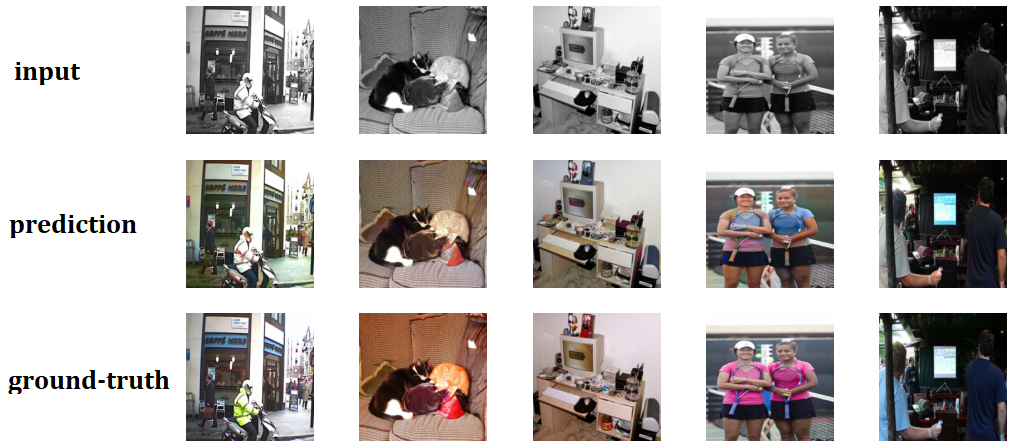
\includegraphics[width=15cm]{images/4_1.png}
\caption{Hình 4.2: Kết quả dự đoán của mô hình GAN với bộ sinh ResNet kết hợp chuẩn 1 trên dữ liệu xác thực của tập dữ liệu \textbf{COCO} sau epoch thứ 15}
\end{figure}

\noindent
Đây là mô hình được huấn luyện dựa vào bộ sinh đã được tiền huấn luyện độc lập trước với 20 epoch, sau đó kết hợp với huấn luyện đối nghịch với bộ phân biệt $70 \times 70$ sau 15 epoch.\\
Kết quả cho thấy rằng mô hình sau khi huấn luyện đã có khả năng tô màu cho các đối tượng trong ảnh, màu ít hoặc gần như không bị lem. Mô hình cũng không dự đoán chính xác tuyệt đối màu của một số đối tượng nhưng hợp lý, theo đúng hướng giải quyết vấn đề mà ta mong muốn.\\

\noindent
Một vài vùng ảnh, mô hình có vẻ như vẫn chưa thực sự tô được màu khi để màu gần giống với mức xám ban đầu. Để lí giải cho hạn chế này, có thể những vùng chưa được tô màu một cách hợp lý là trong quá trình huấn luyện, mô hình chưa được học qua ảnh có bố cục hoặc đối tượng tương tự. Điều này dẫn đến một hạn chế khác nữa, đối với những ảnh có bố cục rõ ràng (ảnh logo), mô hình có thể sẽ không có khả năng tô được màu vì không nhận diện được bối cảnh. Thêm một hạn chế khác là mô hình cũng chưa thực sự biết được những điểm ảnh nào sẽ cùng một đối tượng và cùng màu. Cụ thể như hình ảnh hai cố gái cầm vợt tennis (ảnh thứ 2 từ phía bên phải), phần dưới của áo được tô màu hồng, còn phần trên của áo lại màu xanh. Ở đây, nếu tô cho phần áo màu hồng hay màu xanh thì đều chấp nhận được, nhưng mô hình lại chọn cách tô hai phía của áo, do được chia bởi phần cánh tay thành hai màu sắc khác nhau.

\begin{figure}[h!]
\centering
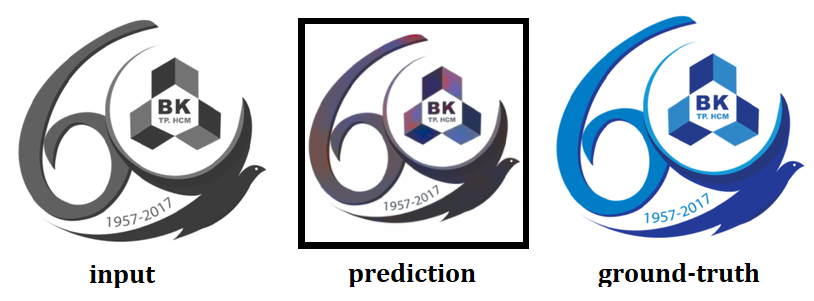
\includegraphics[width=15cm]{images/4_12.PNG}
\caption{Hình 4.3: Mô hình hoàn toàn bế tắc trước logo kỷ niệm 60 năm của trường ĐH Bách Khoa TP.HCM}
\end{figure}

\noindent
Những hạn chế trên, ta hoàn toàn có thể khắc phục bằng cách cho mô hình được huấn luyện thêm với những tập dữ liệu khác. Một hướng khác, ta có thể sử dụng một mạng được huấn luyện trước tốt hơn \textbf{ResNet18} như \textbf{ResNet50}, \textbf{ResNet101} hoặc \textbf{DenseNet} khi giới hạn phần cứng cho phép.

\begin{figure}[h!]
\centering
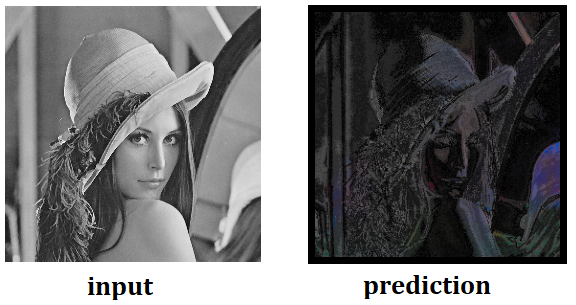
\includegraphics[width=10cm]{images/4_13.png}
\caption{Hình 4.4: Trường hợp đặc biệt khi mô hình làm việc tệ với ảnh có bộ cục đơn giản}
\end{figure}

\noindent
\textbf{Hình 4.4} thực sự là một kết quả bất ngờ mà hiện tại nhóm em vẫn chưa lí giải được tại sao mô hình cho kết quả không thực sự tốt. Việc mô hình không có khả năng làm việc với ảnh mặt người là không khả thi khi ở phần \textbf{4.3 \nameref{compare}} cũng có một ảnh mặt người tương tự và mô hình vẫn cho kết quả ổn. Đây là một trường hợp đặc biệt (\textit{edge case}) cần tìm hiểu thêm.

\subsection{So sánh bộ sinh ResNet trước và khi được huấn luyện đối nghịch}\label{compare}
Việc so sánh giữa hai mô hình này sẽ cho ta cái nhìn về sự ảnh hưởng của mô hình sau khi được huấn luyện đối nghịch. Cụ thể, nhóm em đã chủ động lựa chọn ngẫu nhiên một vài (số lượng 5) tấm ảnh từ Google về ảnh chân dung, phong cảnh, toà nhà cũng như những ảnh có nhiều đối tượng (chi tiết) để thử nghiệm.

\begin{figure}[h!]
\centering
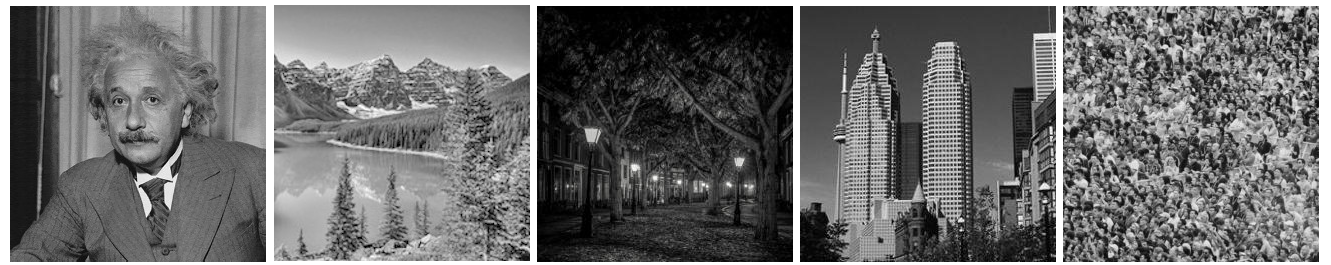
\includegraphics[width=15cm]{images/4_2.PNG}
\caption{Hình 4.5: Những tấm ảnh được lựa chọn để thử nghiệm sự khác biệt}
\end{figure}

\noindent
Trước khi đưa cho mô hình thực hiện tô màu, không khó để đoán được rằng hình ảnh đầu tiên (phía trái ngoài cùng) có ít chi tiết nhất nên sẽ có kết quả tốt nhất. Ngược lại, hình ảnh cuối cùng (phía phải ngoài cùng) có rất nhiều chi tiết nên kết quả khó có thể đạt được tốt như những tấm ảnh ít chi tiết. Và không ngoài dự đoán, kết quả có được khá đúng với những gì mong đợi.

\begin{figure}[h!]
\centering
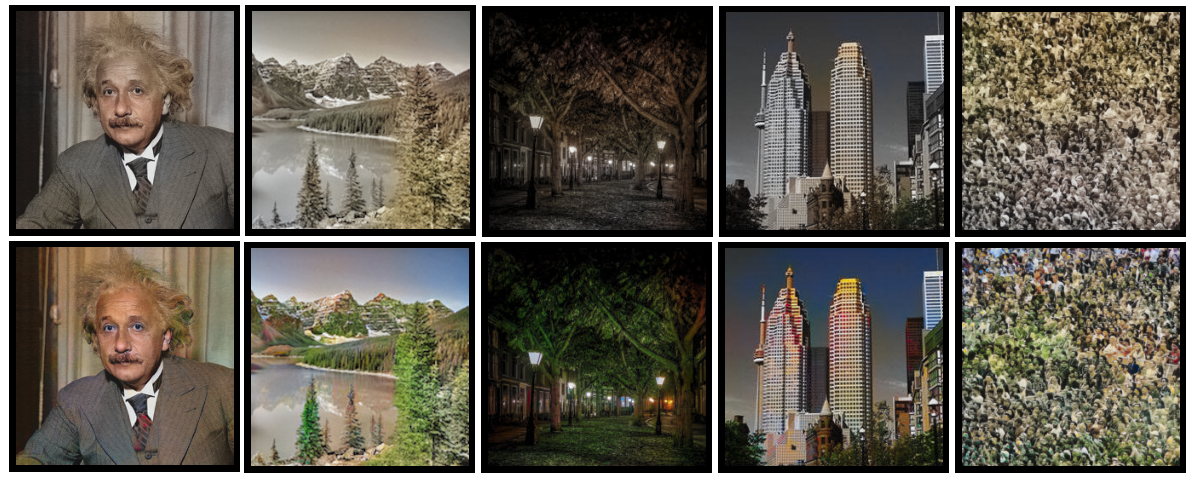
\includegraphics[width=15cm]{images/4_3.PNG}
\caption{Hình 4.6: So sánh kết quả dự đoán của hai mô hình là mô hình chỉ dùng chuẩn 1 (phía trên) với mô hình GAN kết hợp chuẩn 1 (phía dưới)}
\end{figure}

\noindent
Ta có thể thấy trong \textbf{Hình 4.5} rằng mô hình sau khi được huấn luyện theo kiểu GAN cho kết quả có màu tươi sáng, chân thật hơn so với khi ta chỉ dùng chuẩn 1 để huấn luyện. Điều này là do mô hình dùng chuẩn 1 nếu không tìm được màu phù hợp thì sẽ sử dụng giá trị trung bình, tức là giá trị \textbf{(a, b)} $\approx (0, 0)$ vì $-1 \le$ \textbf{a}, \textbf{b} $\le 1$. Khi đó, màu của điểm ảnh sẽ không khác nhiều so với mức xám \textbf{L} đầu vào, khiến cho kết quả của mô hình chỉ dùng chuẩn 1 dường như chỉ thay đổi độ sáng của ảnh đầu vào chứ không thực sự tô được màu. Và hạn chế này đã được khắc phục rất nhiều khi ta đưa mô hình qua huấn luyện đối nghịch (\textit{GAN}).

%%%%%%%%%%%%%%%%%%%%%%%%%%%%%%%%%
\section{Kết luận \& Hướng phát triển}

\subsection{Kết luận}
Về kết quả đề tài, nhóm đã thành công trong việc xây dựng một mô hình có khả năng \textbf{tự động tô màu những ảnh xám, cũ một cách chân thực, hợp lí}. Kiến trúc mô hình là kiến trúc của một \textbf{mạng đối nghịch tạo sinh} với \textbf{bộ phân biệt $70 \times 70$} kết hợp với \textbf{bộ sinh theo kiến trúc mạng Unet} được tạo nên từ phương pháp \textbf{học chuyển tiếp từ mạng ResNet18}.\\

\noindent
Dẫu vậy, mô hình vẫn chưa có kết quả tốt khi áp dụng với những ảnh có bố cục, đối tượng mà mô hình chưa được học trong quá trình huấn luyện. Như đã đề cập ở phần \textbf{4 \nameref{experiment}}, ta hoàn toàn có thể cải thiện trí tuệ mô hình thông qua việc tìm thêm nhiều tập dữ liệu với các bố cục, đối tượng phong phú để huấn luyện thêm hoặc cải thiện bộ sinh bằng cách lựa chọn một mạng có kết nối tắt mạnh mẽ hơn ResNet18.\\
Một cách tiếp cận khác để cải thiện mô hình đó là huấn luyện nhiều bộ sinh, mỗi bộ sinh sẽ đảm nhiệm mỗi chủ đề khác nhau, như vậy chỉ cần cho bộ sinh học những tấm ảnh liên quan đến chủ đề của mình. Bằng việc chuyên môn hoá cho chủ đề của bộ sinh, ta không còn yêu cầu một bộ sinh có thể tô màu tốt cho mọi bố cục tuy nhiên lại giúp quá trình huấn luyện được đơn giản hơn do không phải học quá nhiều và sẽ cho kết quả tốt hơn cả khi được đưa cho ảnh đúng chuyên môn.\\

\noindent
So với mục tiêu đề ra trong phần \textbf{1.2 \nameref{objective}}, khi xây dựng một mô hình dự đoán được màu của những đối tượng trong ảnh xám một cách hợp lí, chất lượng không yêu cầu phải tốt như làm thủ công, giúp tiết kiệm thời gian trong quá trình phục hồi màu cho ảnh xám thì mô hình đã xử lí được vấn đề được nêu ra.\\

\noindent
Sau quá trình tìm hiểu và hoàn thành đề tài, bản thân nhóm đã học thêm được nhiều kiến thức về những không gian màu của ảnh số ngày nay (RGB, Lab). Thêm vào đó, nhờ việc thực sự đắm mình vào học sâu (\textit{dive into deep learning}), nhóm em đã có một cái nhìn rõ ràng hơn về học máy/học sâu trong một mảng khổng lồ như là \textbf{trí tuệ nhân tạo}.

\subsection{Hướng phát triển}
Đề tài có thể được áp dụng để làm những tác vụ liên quan đến phục chế màu cho ảnh xám, bị mất màu hoặc ảnh cũ, thời chiến tranh. Giúp cho quá trình phục chế được tiết kiệm thời gian. Kết hợp với tinh chỉnh bằng phương pháp thủ công, ta hoàn toàn có thể có những kết quả phục chế đẹp đẽ và cũng nhanh chóng.\\

\noindent
Không chỉ dừng lại ở hình ảnh, ta cũng có thể áp dụng mô hình để phục chế màu cho các video, vì bản chất một video là sự kết hợp từ nhiều khung hình (\textit{frame}) ghép lại. Trong thư mục \texttt{test\_results}\footnote{Được chứa trong thư mục \href{https://github.com/dee-ex/EE3151\_SEM202\_PROJECT}{https://github.com/dee-ex/EE3151\_SEM202\_PROJECT}} có kết quả thử nghiệm của mô hình qua việc phục chế màu một đoạn nhỏ về một phóng sự về chiến tranh ở Việt Nam.

\begin{figure}[h!]
\centering
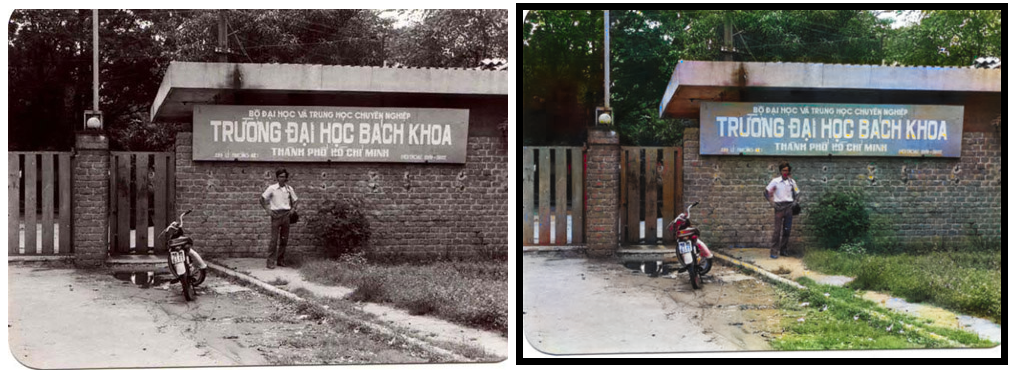
\includegraphics[width=14cm]{images/5_1.PNG}
\caption{Hình 5.1: Ảnh Trường ĐH Bách Khoa TP.HCM ngày xưa (trái) và sau khi tô màu (phải)}
\end{figure}

\clearpage

%%%%%%%%%%%%%%%%%%%%%%%%%%%%%%%%%
\section{Phục lục - Ảnh màu}

\begin{figure}[h!]
\centering
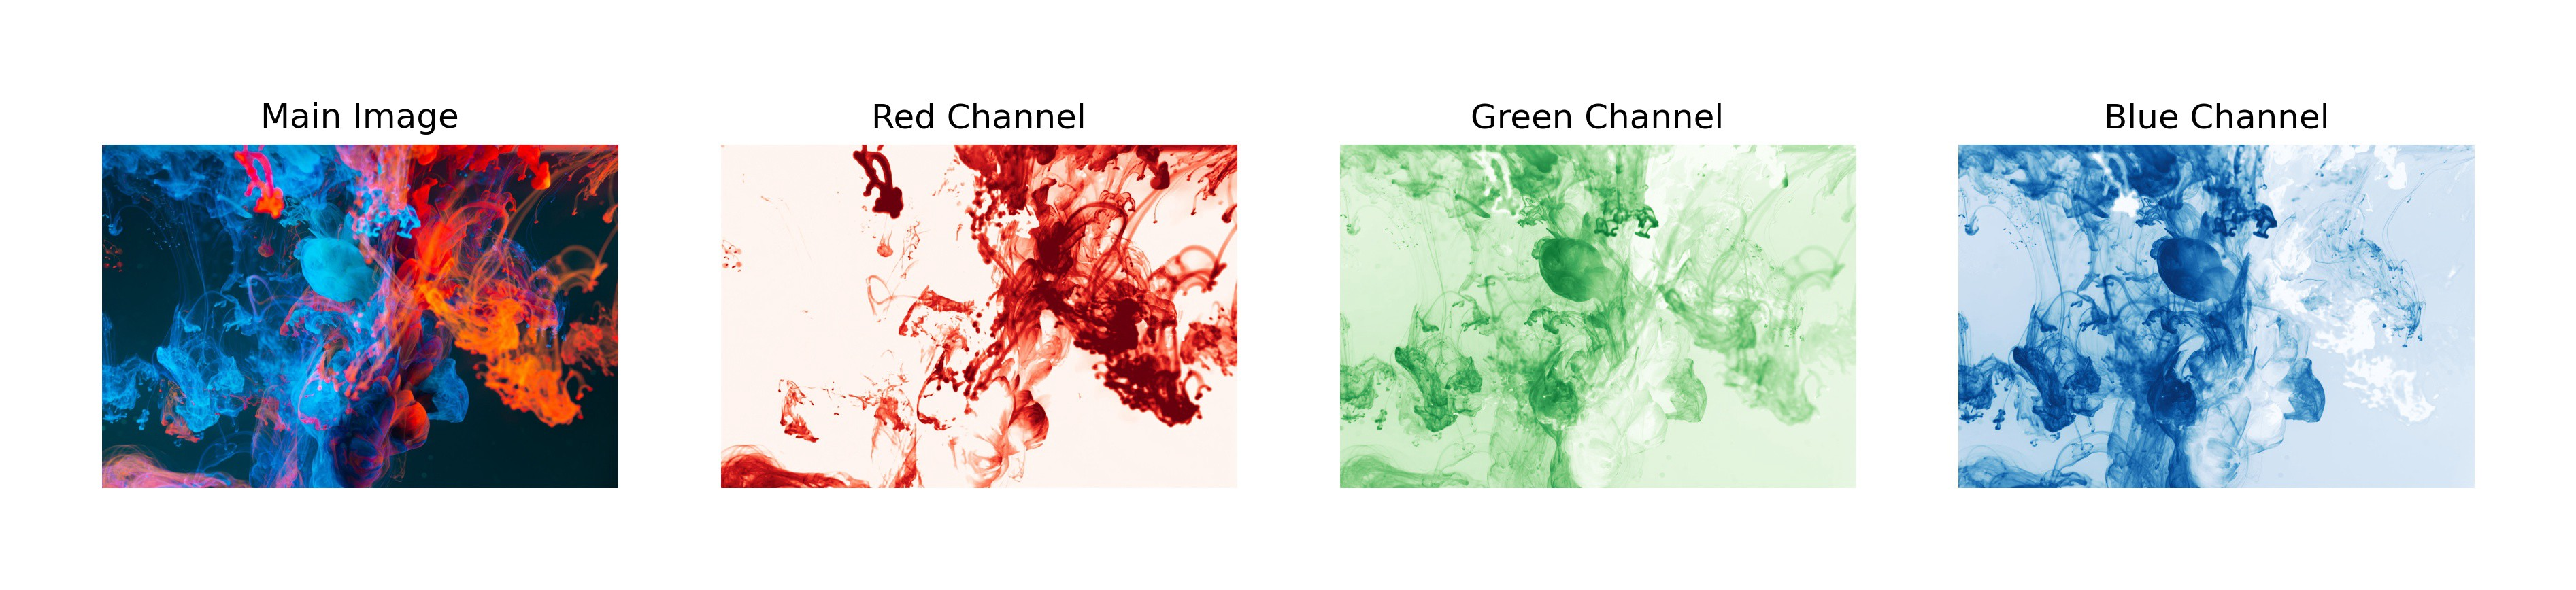
\includegraphics[width=14cm]{images/2_1.jpeg}
\caption*{Hình 2.1: Các kênh màu đỏ, lục và lam được tách ra riêng biệt. Nguồn: \href{https://bit.ly/3eKaaBj}{https://bit.ly/3eKaaBj}}
\end{figure}

\begin{figure}[h!]
\centering
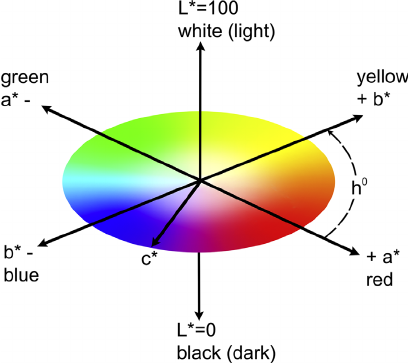
\includegraphics[width=5cm]{images/2_2.png}
\caption*{Hình 2.2: Không gian màu Lab. Nguồn: \href{https://bit.ly/3nFIQIp}{https://bit.ly/3nFIQIp}}
\end{figure}

\begin{figure}[h!]
\centering
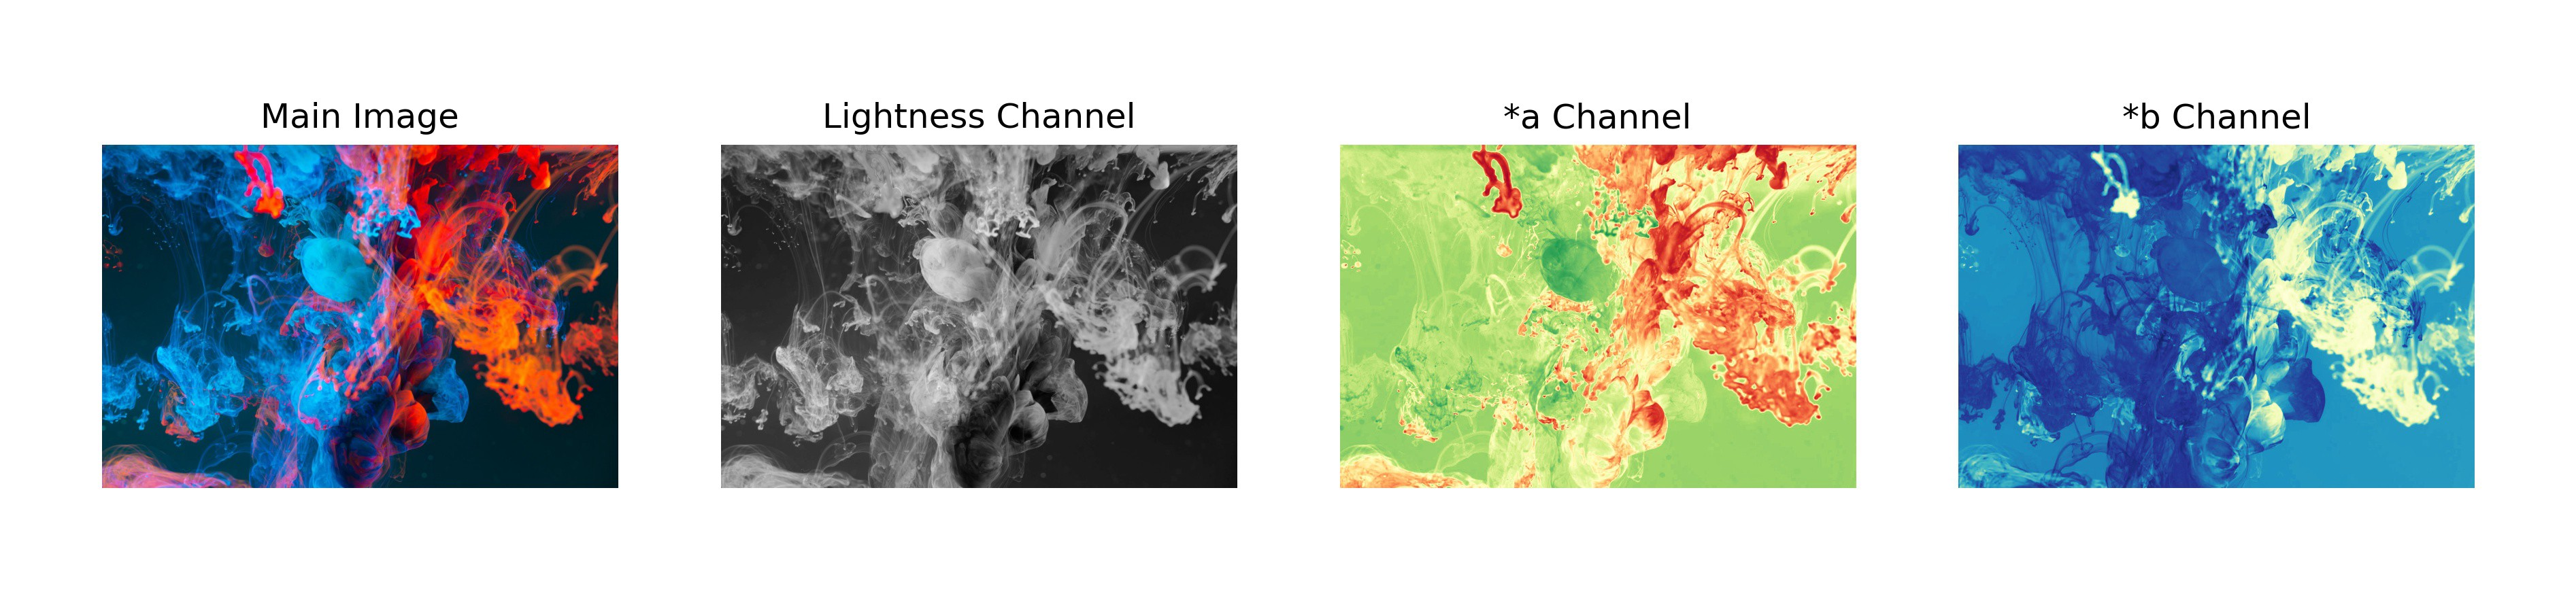
\includegraphics[width=14cm]{images/2_3.jpeg}
\caption*{Hình 2.3: Các giá trị \textbf{L}, \textbf{a} và \textbf{b} được tách ra riêng biệt. Nguồn: \href{https://bit.ly/3eKaaBj}{https://bit.ly/3eKaaBj}}
\end{figure}

\begin{figure}[h!]
\centering
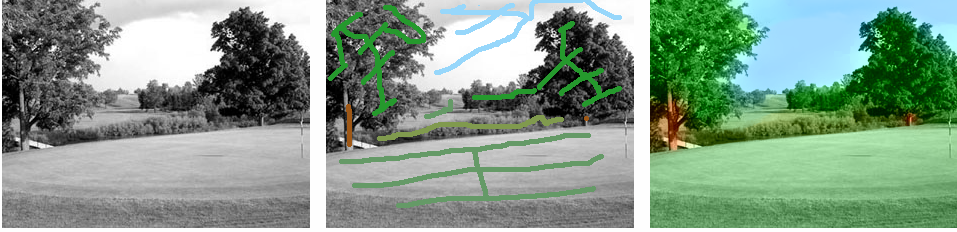
\includegraphics[width=11cm]{images/2_4.png}
\caption*{Hình 2.4: Mô tả ý tưởng thuật toán đánh dấu vài điểm ảnh. Nguồn: \href{https://bit.ly/3eKdmwN}{https://bit.ly/3eKdmwN}}
\end{figure}

\begin{figure}[h!]
\centering
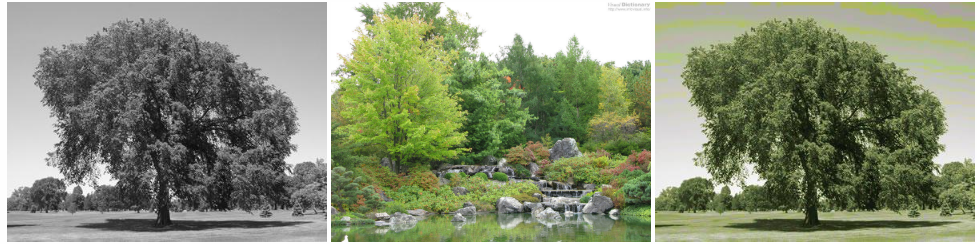
\includegraphics[width=11cm]{images/2_5.png}
\caption*{Hình 2.5: Mô tả ý tưởng thuật toán ảnh có bố cục tương tự. Nguồn: \href{https://bit.ly/3eKdmwN}{https://bit.ly/3eKdmwN}}
\end{figure}

\begin{figure}[h!]
\centering
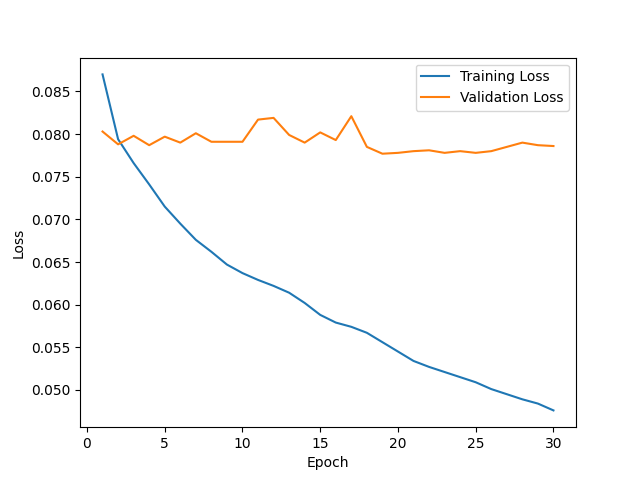
\includegraphics[width=7cm]{images/3_5.png}
\caption*{Hình 3.5: Giá trị mất mát của bộ sinh trên hai tập huấn luyện \& xác thực qua từng epoch}
\end{figure}

\begin{figure}[h!]
\centering
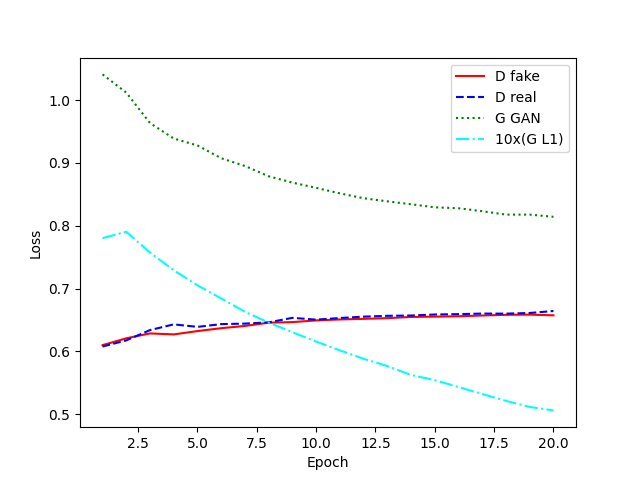
\includegraphics[width=7cm]{images/3_6.png}
\caption*{Hình 3.6: Giá trị các thành phần mất mát của của bộ phân biệt và bộ sinh qua từng epoch}
\end{figure}

\begin{figure}[h!]
\centering
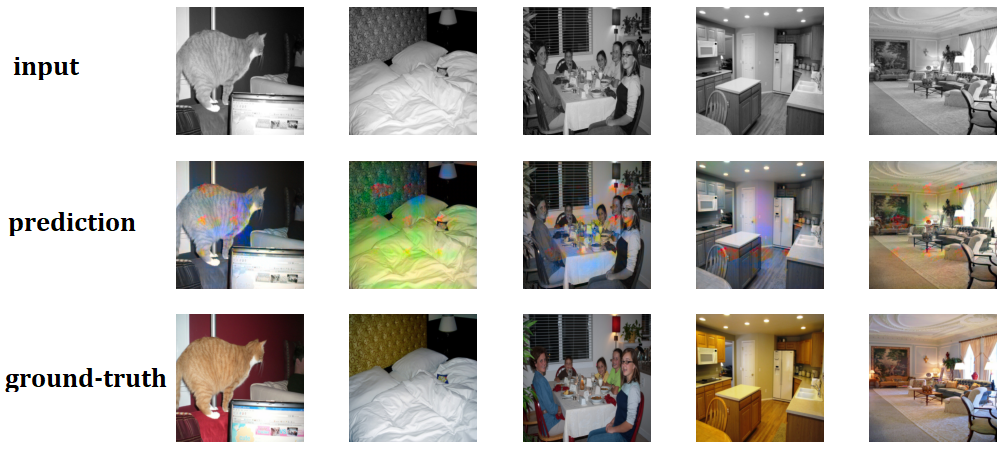
\includegraphics[width=10.5cm]{images/4_0.png}
\caption*{Hình 4.1: Kết quả dự đoán của mô hình GAN với bộ sinh đơn giản kết hợp chuẩn 1 trên dữ liệu xác thực của tập dữ liệu \textbf{COCO} sau epoch thứ 34}
\end{figure}

\begin{figure}[h!]
\centering
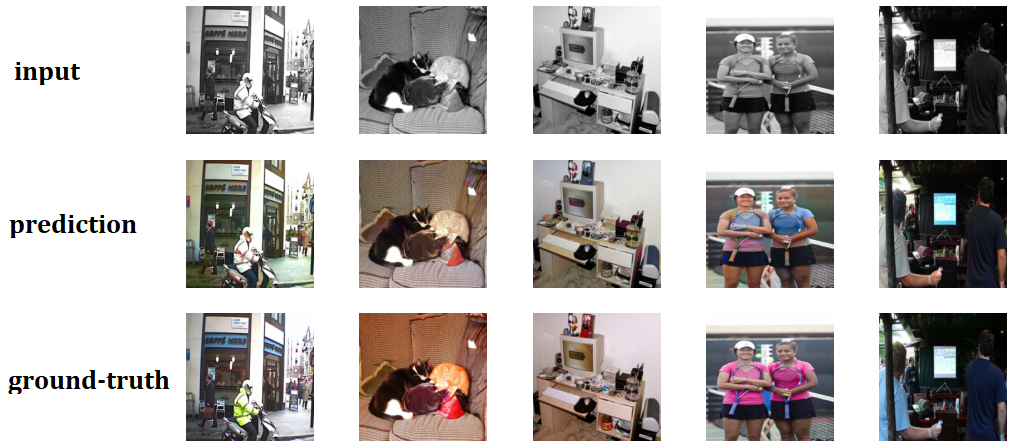
\includegraphics[width=10.5cm]{images/4_1.png}
\caption*{Hình 4.2: Kết quả dự đoán của mô hình GAN với bộ sinh ResNet kết hợp chuẩn 1 trên dữ liệu xác thực của tập dữ liệu \textbf{COCO} sau epoch thứ 15}
\end{figure}

\begin{figure}[h!]
\centering
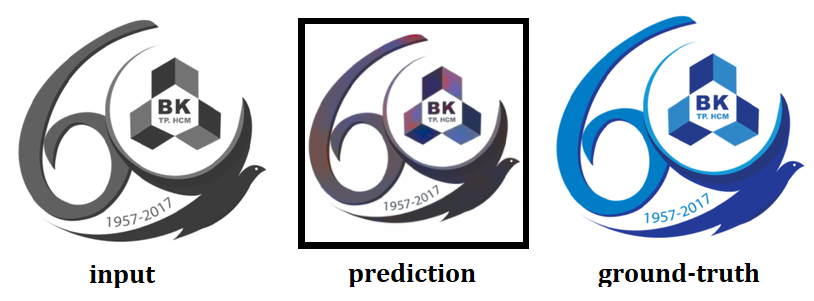
\includegraphics[width=8cm]{images/4_12.PNG}
\caption*{Hình 4.3: Mô hình hoàn toàn bế tắc trước logo kỷ niệm 60 năm của trường ĐH Bách Khoa TP.HCM}
\end{figure}

\begin{figure}[h!]
\centering
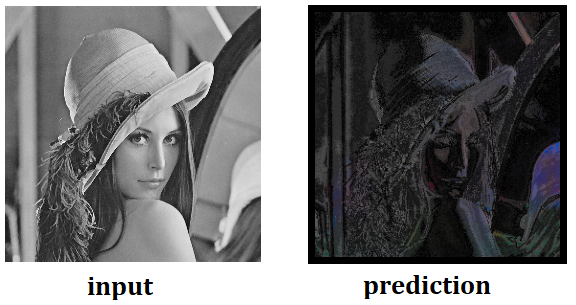
\includegraphics[width=8cm]{images/4_13.png}
\caption*{Hình 4.4: Trường hợp đặc biệt khi mô hình làm việc tệ với ảnh có bộ cục đơn giản}
\end{figure}

\begin{figure}[h!]
\centering
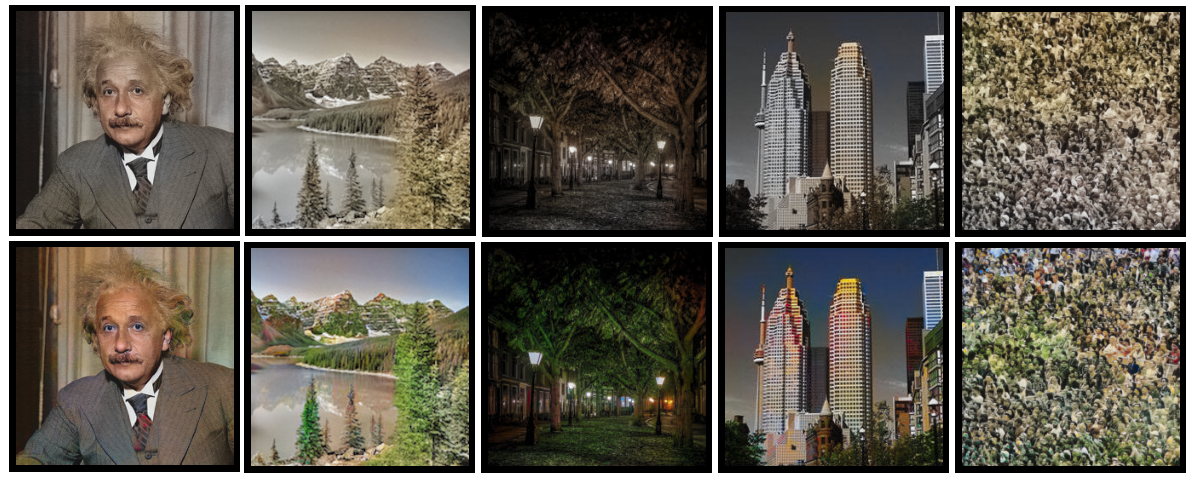
\includegraphics[width=14cm]{images/4_3.PNG}
\caption*{Hình 4.6: So sánh kết quả dự đoán của hai mô hình là mô hình chỉ dùng chuẩn 1 (phía trên) với mô hình GAN kết hợp chuẩn 1 (phía dưới)}
\end{figure}

\begin{figure}[h!]
\centering
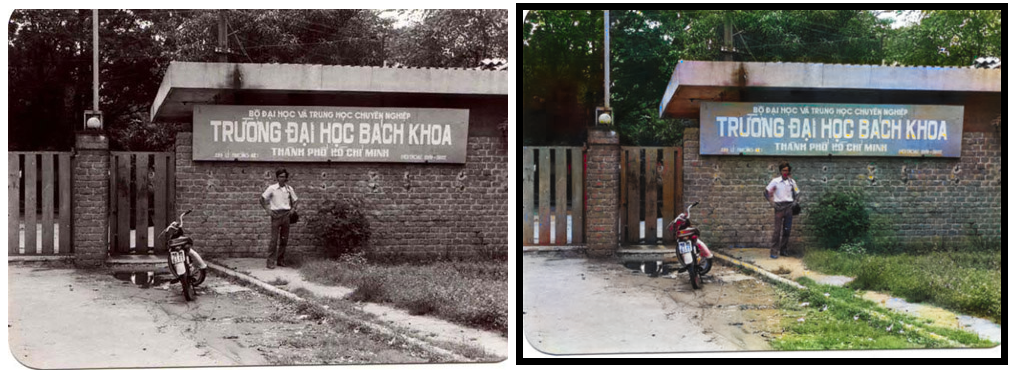
\includegraphics[width=17cm]{images/5_1.PNG}
\caption*{Hình 5.1: Ảnh Trường ĐH Bách Khoa TP.HCM ngày xưa (trái) và sau khi tô màu (phải)}
\end{figure}

\clearpage

\renewcommand{\refname}{Tài liệu tham khảo}
%%%%%%%%%%%%%%%%%%%%%%%%%%%%%%%%%
\begin{thebibliography}{80}\label{references}

    \bibitem{aladdinpersson} Aladdin Persson, ``Building our first simple GAN'', \href{https://youtu.be/OljTVUVzPpM}{https://youtu.be/OljTVUVzPpM}, (2020).

    \bibitem{aladdinpersson} Aladdin Persson, ``Pix2Pix Paper Walkthrough'', \href{https://youtu.be/SuddDSqGRzg}{https://youtu.be/SuddDSqGRzg}, (2021).

    \bibitem{aladdinpersson} Aladdin Persson, ``Pix2Pix implementation from scratch'', \href{https://youtu.be/SuddDSqGRzg}{https://youtu.be/SuddDSqGRzg}, (2021).

    \bibitem{aladdinpersson} Aladdin Persson, ``U-NET Paper Walkthrough'', \href{https://youtu.be/oLvmLJkmXuc}{https://youtu.be/oLvmLJkmXuc}, (2021).
    
    \bibitem{astonzhang} Aston Zhang, Zachary C. Lipton, Mu Li, and Alexander J. Smola, ``Dive into Deep Learning'', (2021).
    
    \bibitem{christopher} Christopher Thomas BSc Hons. MIAP, ``U-Nets with ResNet Encoders and cross connections'', \href{https://bit.ly/3ttEu8x}{https://bit.ly/3ttEu8x}, (2019).

    \bibitem{connorshorten} Connor Shorten, ``DCGANs (Deep Convolutional Generative Adversarial Networks)'',\\ \href{https://bit.ly/3nFC7OC}{https://bit.ly/3nFC7OC}, (2018).

    \bibitem{cornorshorten} Cornor Shorten, ``Pix2Pix'', \href{https://bit.ly/3eMDGGt}{https://bit.ly/3eMDGGt}, (2019).

    \bibitem{elistevens} Eli Stevens, Luca Antiga, Thomas Viehmann and Foreword by Soumith Chintala, ``Deep Learning with PyTorch'', Manning Publications, New York (2020).

    \bibitem{emilwallner} Emil Wallner, ``How to colorize black \& white photos with just 100 lines of neural network code'', \href{https://bit.ly/3u8uSkN}{https://bit.ly/3u8uSkN}, (2017).

    \bibitem{harshalllamba} Harshall Lamba, ``Understanding Semantic Segmentation with UNET'', \href{https://bit.ly/3tdDK7B}{https://bit.ly/3tdDK7B}, (2019).

    \bibitem{goodfellow} Ian J. Goodfellow et al. ``Generative Adversarial Networks'', \href{https://arxiv.org/abs/1406.2661}{https://arxiv.org/abs/1406.2661}, (2014).

    \bibitem{jasonbrownlee} Jason Brownlee, ``A Gentle Introduction to Pix2Pix Generative Adversarial Network'',\\ \href{https://bit.ly/2RhbbsC}{https://bit.ly/2RhbbsC}, (2019).

    \bibitem{josephrocca} Joseph Rocca, ``Understanding Generative Adversarial Networks (GANs)'', \href{https://bit.ly/3vzdPIU}{https://bit.ly/3vzdPIU}, (2019).

    \bibitem{juan} Juan, ``What range does skimage use in LAB color space for each channel?'', \href{https://bit.ly/3eaonbt}{https://bit.ly/3eaonbt}, (2020).

    \bibitem{mehdimirza} Mehdi Mirza \& Simon Osindero, ``Conditional Generative Adversarial Nets'',\\ \href{https://arxiv.org/abs/1411.1784}{https://arxiv.org/abs/1411.1784}, (2014).

    \bibitem{moeinshariatnia} Moein Shariatnia, ``Colorizing black \& white images with U-Net and conditional GAN — A Tutorial'', \href{https://bit.ly/3eKaaBj}{https://bit.ly/3eKaaBj}, (2020).

    \bibitem{olafronneberger} Olaf Ronneberger, Philipp Fischer \& Thomas Brox, ``U-Net: Convolutional Networks for Biomedical Image Segmentation'', \href{https://arxiv.org/abs/1505.04597}{https://arxiv.org/abs/1505.04597}, (2015)

    \bibitem{phamdinhkhanh} Pham Dinh Khanh, ``Image Segmentation'', \href{https://bit.ly/335IEZE}{https://bit.ly/335IEZE}, (2020).

    \bibitem{phillipisola} Phillip Isola, Jun-Yan Zhu, Tinghui Zhou \& Alexei A. Efros, ``Image-to-Image Translation with Conditional Adversarial Networks'', \href{https://arxiv.org/abs/1611.07004}{https://arxiv.org/abs/1611.07004}, (2016).

    \bibitem{richardzhang} Richard Zhang, Phillip Isola \& Alexei A. Efros, ``Colorful Image Colorization'',\\ \href{https://arxiv.org/abs/1603.08511}{https://arxiv.org/abs/1603.08511}, (2016).

    \bibitem{sahil} Sahil, ``Understanding PatchGAN'', \href{https://bit.ly/3xJy0Wo}{https://bit.ly/3xJy0Wo}, (2020).

    \bibitem{trungthanhnguyen} Trung Thanh Nguyen, ``Auto Colorize Grayed Image With Deep Learning'', \href{https://bit.ly/3theTj4}{https://bit.ly/3theTj4}, (2018).

    \bibitem{tuannguyen} Tuan Nguyen, ``Conditional GAN (cGAN)'', \href{https://bit.ly/3udFFKH}{https://bit.ly/3udFFKH}, (2020).

    \bibitem{tuannguyen} Tuan Nguyen, ``Deep Convolutional GAN (DCGAN)'', \href{https://bit.ly/3uhxtcb}{https://bit.ly/3uhxtcb}, (2020).

    \bibitem{tuannguyen} Tuan Nguyen, ``Giới thiệu về GAN'', \href{https://bit.ly/3aXhHvD}{https://bit.ly/3aXhHvD}, (2019).

    \bibitem{tuannguyen} Tuan Nguyen, ``Pix2pix'', \href{https://bit.ly/3xGVR9h}{https://bit.ly/3xGVR9h}, (2020).
    
    \bibitem{wiki} Wikipedia, ``CIELAB color space'', \href{https://en.wikipedia.org/wiki/CIELAB\_color\_space}{https://en.wikipedia.org/wiki/CIELAB\_color\_space}, (2021).

\end{thebibliography}
\end{document}